% Sample file for JNLP (Journal of Natural Language Processing)
% English Paper.
% For ASCII pLaTeX2e
% This file requires
%	jnlp_3.3.cls
% For e_yourrefs.bib, jbibtex requires
%	jnlpbbl_2.1.bst

%%%%%%%%%%%%%%%%%%%%%%%%%%%%%%%%%%%%%%%%%%%%%%%%%%%%%%%%%%%%%%%%%%%%%%%%%
%%%% Please do not appoint other files.                              %%%%
%%%% But I do not mind when I had you dispatch it with an article.   %%%%
%%%% In this case a thing working in ASCII pLaTeX is best.           %%%%
%%%%%%%%%%%%%%%%%%%%%%%%%%%%%%%%%%%%%%%%%%%%%%%%%%%%%%%%%%%%%%%%%%%%%%%%%

% 16-Nov-20 by Nakanishi Printing Co., Ltd
% 13-Apr-20 by masayu-a@ninjal.ac.jp (for jother.tex, eother.tex)
% 27-Dec-17 by Nakanishi Printing Co., Ltd
% 07-Sep-06 by Nakanishi Printing Co., Ltd (for Platex2e)
% 13-Jan-95 by m_yama@pluto.ai.kyutech.ac.jp (renamed from theapa to nlpbbl)
% 30-Nov-94 by nakamura@ai.kyutech.ac.jp, acknowledgment example
% 08-Nov-94 by nakamura@ai.kyutech.ac.jp, copyright
% 06-Nov-94 by nakamura@ai.kyutech.ac.jp

%%%%%%%%%%%%%%%%%%%%%%%%%%%%%%%%%%%%%%%%
\documentclass[english,tombow]{jnlp_3.3}
\usepackage{jnlpbbl_2.1}
%%%% Citation Format
%% \cite{Article_01} -> "(LastName 2006)"
%% \citeA{Article_01} -> "LastName (2006)" 

% \usepackage[thai,english,main=japanese]{babel}
% \usepackage[utf8x]{inputenc}
% \newcommand\thai[1]{{\begin{otherlanguage}{english}#1\end{otherlanguage}}}

\usepackage[dvipdfmx, nosetpagesize]{graphicx}
\usepackage[dvipdfmx]{xcolor}
% \usepackage[dvipsnames]{xcolor}
\usepackage{amsmath,amsfonts}
\usepackage{url}
\renewcommand\UrlFont{\rmfamily}

% my packages
%% for Thai text
% \usepackage[thai,english,main=japanese]{babel}
% \usepackage[utf8x]{inputenc}
% \newcommand\thaitext[1]{{\begin{otherlanguage}{english}#1\end{otherlanguage}}}

%% normal packages
\usepackage{nccmath}
\usepackage{amssymb}
\usepackage{float}
\usepackage{booktabs}
\usepackage{multirow}
\usepackage{subfiles}
\usepackage{xcolor}
\usepackage{subcaption}
\usepackage{arydshln}  % dashed line

% my commands
\newcommand{\draft}[1]{\textcolor{gray}{#1}}
\newcommand{\verify}[1]{\textcolor{red}{#1}}
\makeatletter
\def\blfootnote{\xdef\@thefnmark{}\@footnotetext}
\makeatother

%%%% Following settings will be edited by editors.
\Volume{}
\Number{}
\Month{}
\Year{2022}
\Issuetitle{Special Issue: XXXXXXXX}

\received{2005}{1}{2}
\revised{2006}{3}{4}
\rerevised{2006}{5}{6}
\accepted{2006}{7}{8}

\setcounter{page}{1}

%%%%%%%%%%%%%%%%%%%%%%%%%%%%%%%%%%%%%%%%%
%%%%   Title, Author, etc.            %%%
%%%%%%%%%%%%%%%%%%%%%%%%%%%%%%%%%%%%%%%%%
\esubject{General Paper}
\etitle{Character-based Thai Word Segmentation with Multiple Attentions}
\eauthor{Thodsaporn Chay-intr\affiref{lrlab} \and Hidetaka Kamigaito\affiref{naist} \and Manabu Okumura\affiref{lrlab-fac}} 
% \eabstract{
% 	Word segmentation is one of early steps in natural language processing (NLP) for most Asian languages, such as Thai, Japanese, and Chinese. 
%
A combination of characters, a fundamental unit, can form into new words with different roles, meanings or grammatical properties.
%
Failing to segment word boundaries precisely tends to affect the performance of the downstream tasks consequently.
%
Thai running text has neither essential word boundaries nor sentence periods.
%
However, spaces are arbitrarily allowed to separate words, phrases, clauses, and sentences.
%
These characteristics make word segmentation in Thai more difficult than in other languages, such as English, German, and Finnish, which have spaces and periods to identify word- and sentence-boundary, respectively.
%

Thai word segmentation can be categorized as a sequence-labeling task that assigns a word-boundary label to each character from a character sequence.
%
Each character can be assigned by specific tagging-scheme, for example, a fine-grained tagging scheme, i.e., BIES (beginning, inside, end, and singleton) \cite{Xue2003}, as shown in Figure~\ref{fig:thbies}.
%
In addition, several tagging schemes, for instance, character- and word-level, have been additionally used to avoid overestimation in domain-adaptation scenarios  \cite{limkonchotiwat-etal-2020-domain,limkonchotiwat-etal-2021-handling}.
\begin{figure}
    \centering
    \begin{subfigure}{0.59\textwidth}
        \centering
        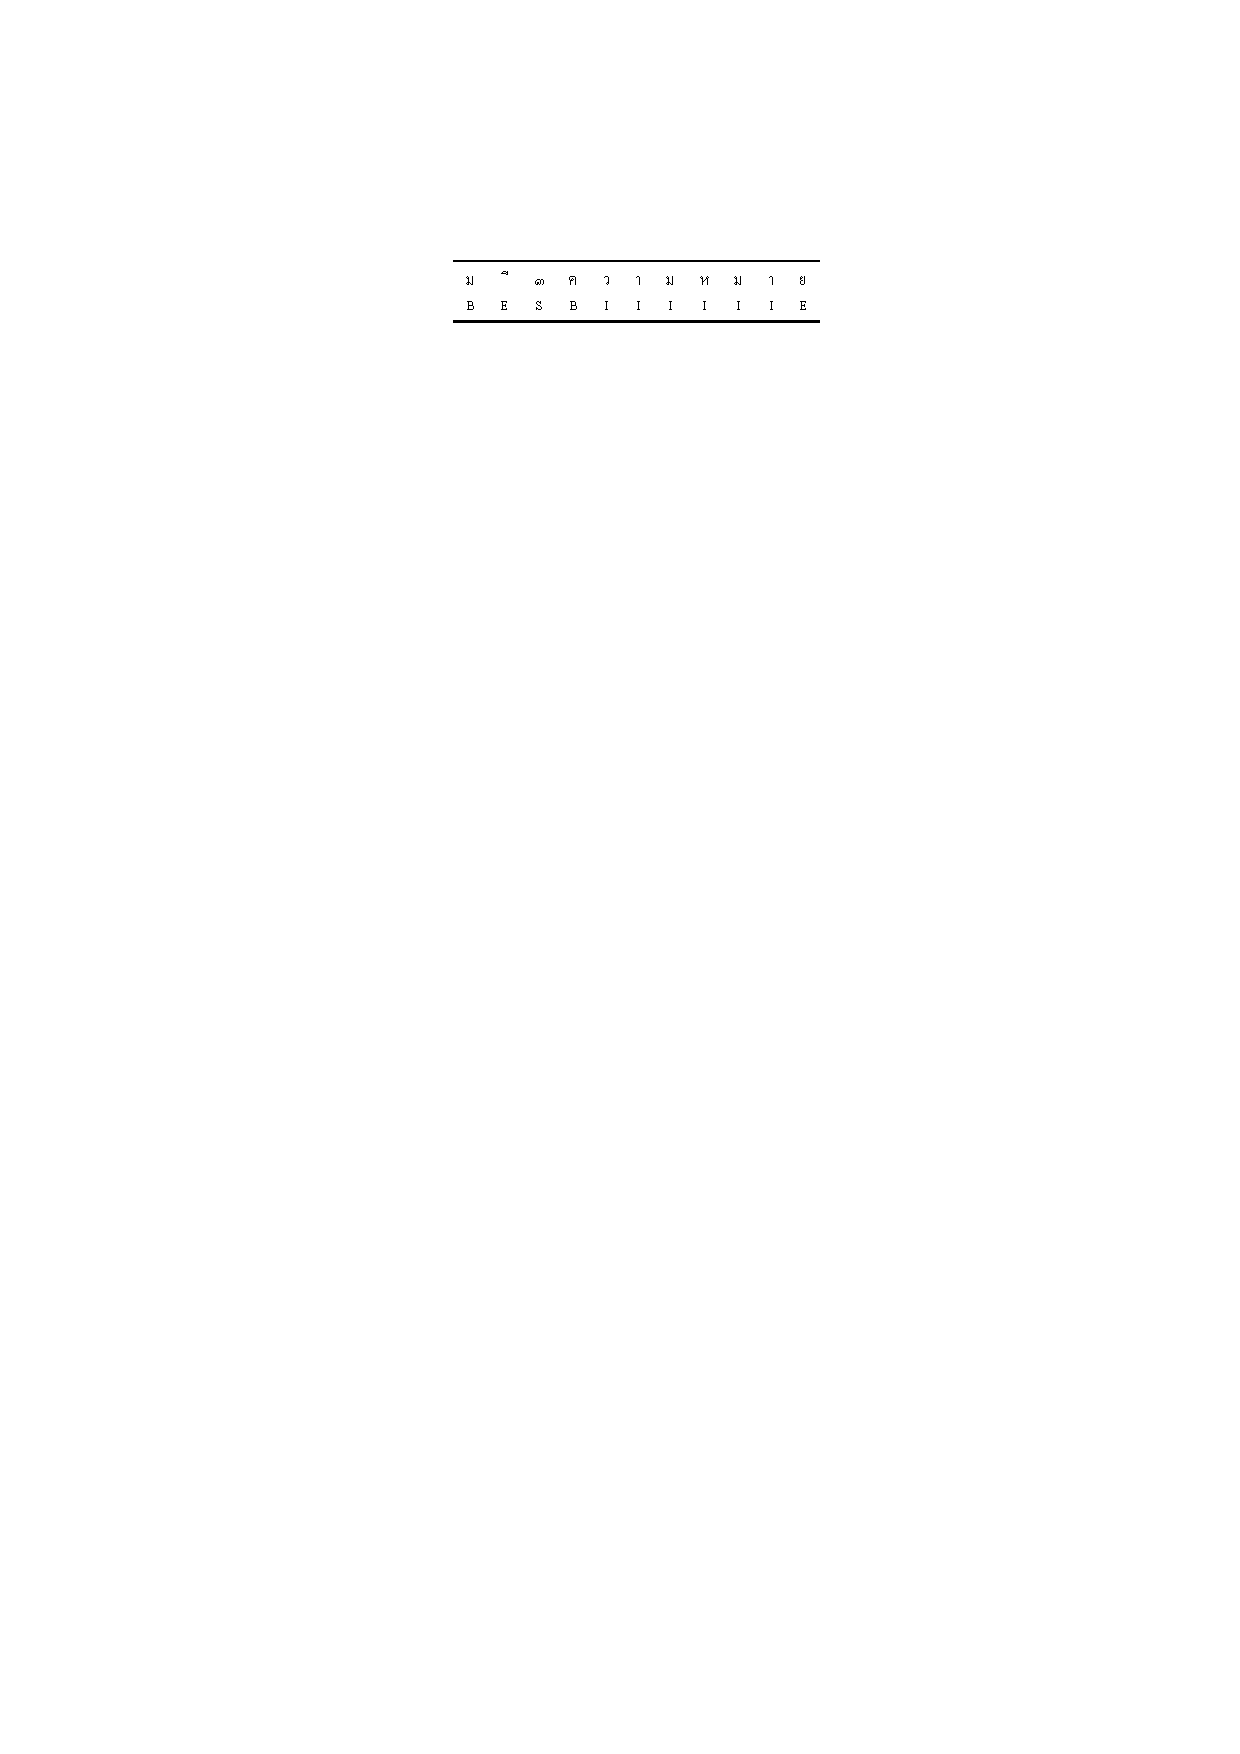
\includegraphics[width=\textwidth]{figures/fig-thbies.pdf}
    \end{subfigure}
    \hspace{\textwidth}
    \begin{subfigure}{0.24\textwidth}   
        \centering
        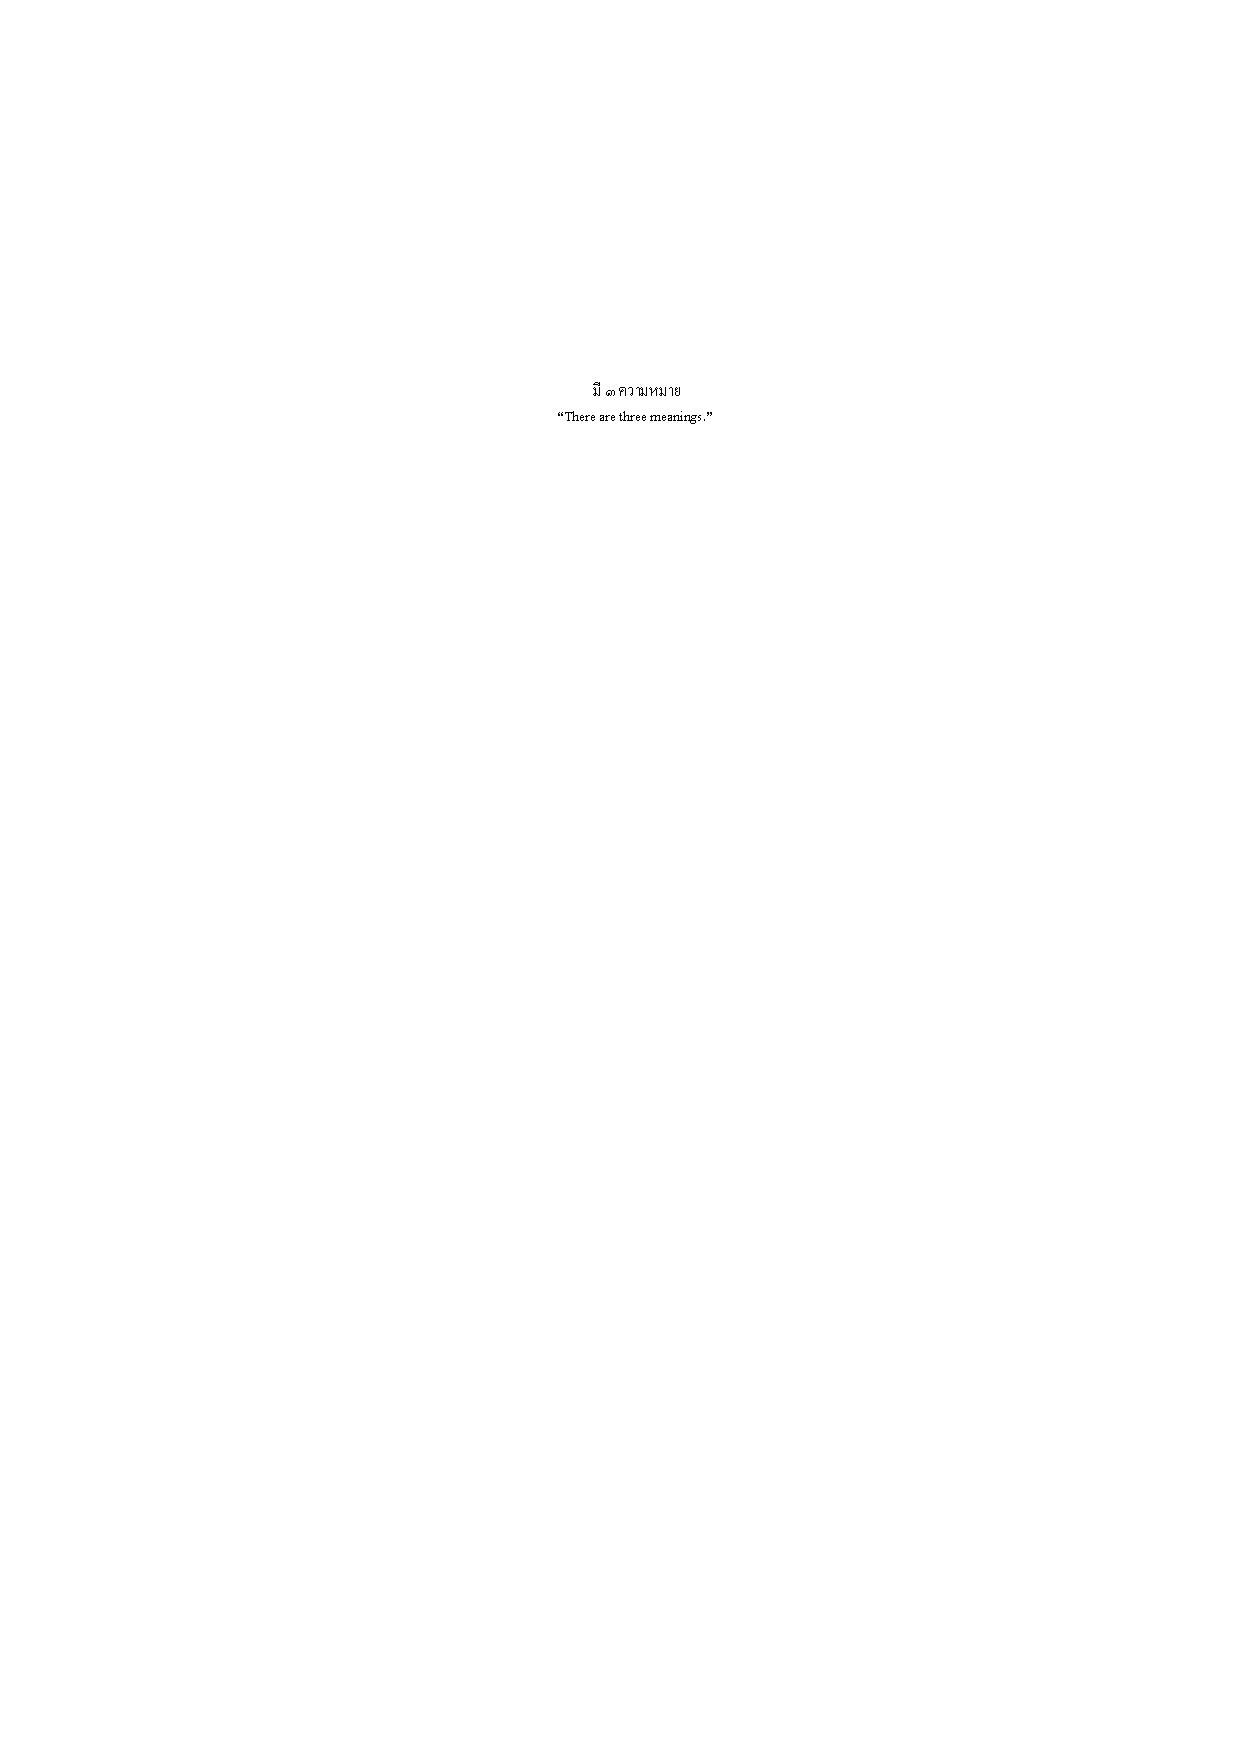
\includegraphics[width=\textwidth]{figures/fig-thbies-tran.pdf}
    \end{subfigure}
    \caption{Thai word segmentation as sequence-labeling task on BIES (beginning, inside, end, and singleton) tagging scheme.}
    \label{fig:thbies}
\end{figure}
%

Neural-network models have been applied and perform well on character-based Thai word segmentation.
%
\citeA{Jousimo2017} applied bidirectional recurrent neural networks with gated recurrent units (GRUs), while \citeA{Chormai2019} proposed an AttaCut \cite{Chormai2019},\footnote{https://github.com/PyThaiNLP/attacut} a convolutional-neural-network (CNN)-based model that mainly provides faster and more accurate word inferring motivated by DeepCut \cite{Kittinaradorn2019}.
%
% See Appendix~\ref{appx:thai-wordseg} for more details.
%
Despite the fact that neural-network models with linguistic knowledge can perform almost perfectly, adapting models with pre-trained neural networks, such as word vectors and language models, is still useful \cite{Shao2018,yan-etal-2020-bert}.
%

In spite of that a pre-trained model (PTM) such as BERT \cite{devlin-etal-2019-bert} has also been successfully applied for word segmentation mostly on Chinese datasets \cite{yang-etal-2019-bert,qiu-etal-2020-concise,ke-etal-2020-unified,huang-etal-2020-towards,ke-etal-2021-pre}, only \citeA{seeha-etal-2020-thailmcut} proposed a transfer-learning approach for Thai word segmentation by pre-training language model on the basis of character-level for character-based word segmentation. 
%
Although it exhibited state-of-the-art performance regarding Thai, it merely uses characters and does not use other information such as word and subword \cite{sennrich-etal-2016-neural,kudo-2018-subword}.
%
However, relying on the transfer-learning method can interact only input and output layers of the models, as known as black boxes, which is considered as its limitation \cite{limkonchotiwat-etal-2020-domain}. 
%
\citeA{limkonchotiwat-etal-2020-domain,limkonchotiwat-etal-2021-handling} proposed alternative approaches to particularly focus on domain-dependent word segmentation to lessen the black box limitation in the transfer learning.
%
Their works could obtain comparable results as the transfer learning method.
%

Additional linguistic-knowledge other than a character sequence, e.g., word, subword, and Thai character clusters (CCs) \cite{Theeramunkong2000} has also been successfully used for word segmentation and downstream tasks \cite{Sutantayawalee2015,Lapjaturapit2018,Nararatwong2018,yang-etal-2019-subword,li-etal-2019-word-segmentation}.
%
Furthermore, an attention mechanism \cite{Bahdanau2015} has been effectively applied to various downstream tasks, particularly a character-based sequence-labeling task that exploit more than one linguistic knowledge \cite{higashiyama-etal-2019-incorporating,tian-etal-2020-joint}.
%

To exploit multiple linguistic-knowledge, we propose a character-based Thai word-segmentation model with multiple attentions that jointly uses corresponding words, CCs, and subwords.
%
Our model is based on the bidirectional long short-term memory with conditional random field (BiLSTM-CRF) architecture, which is the baseline model for this study, because it has been successfully applied in sequence-labeling tasks for Thai and other languages \cite{Jousimo2017,Nararatwong2018,higashiyama-etal-2019-incorporating,seeha-etal-2020-thailmcut,tian-etal-2020-joint}.

%
Furthermore, Transformer-based PTM has not been incorporated in Thai word segmentation.
%
Thus, we additionally expand potential of using a pre-trained model, particularly Transformer-based PTM, in Thai word segmentation by applying BERT into our model.
%
To our best knowledge, this work is the first to adopts PTM in Thai word segmentation. 

Our contributions are as follows:
%
\begin{itemize}
    \setlength\itemsep{0.01em}
    \item We use word, CC, and subword with multiple attentions to estimate the relationships of characters in character-based Thai word segmentation.
    \item We conduct experiment for showing the validity of using CC over subword units in terms of segmentation performance and a segmentation result that does not violate Thai writing system.
    \item Our model shows improvement over the baseline model and outperforms previous works in Thai word segmentation.
    \item Our proposed model outperforms recent works that focus domain-dependent word segmentation on Thai domain-dependent datasets.
    \item We incorporate Multilingual BERT into character-based Thai word segmentation, and conduct a comparison between our BiLSTM-based model and BERT-based model. Moreover, we found that most of BERT-incorporated model could not outperform our proposed BiLSTM-based model.
    \item Our code is publicly available.\footnote{\url{https://github.com/tchayintr/thwcc-attn}}
\end{itemize}
% }
% \ekeywords{Thai word segmentation, representation learning}
\eabstract{%
	Character-based word-segmentation models have been extensively applied to agglutinative languages, including Thai, due to their high performance. 
%
These models estimate word boundaries from a character sequence.
%
However, a Thai character unit in sequences has no essential meaning, compared with word, subword, and character cluster units that represent meaningful-linguistic knowledge.
%
We propose a Thai word-segmentation model that uses various types of information, including words, subwords, and character clusters, from a character sequence.
%
Our model applies multiple attentions to refine segmentation inferences by estimating the significant relationships among characters and various unit types.
%
We evaluate our model on three Thai datasets, and our experimental results show that our model outperforms other Thai word-segmentation models as well as showing the validity of using character-cluster over subword.
%
Furthermore, according to our analysis, particularly case study, our model can segment accurate results while compared models yield incorrect results that violate Thai writing system.
}
\ekeywords{Thai word segmentation, representation learning}

\headauthor{Chay-intr et al.}
\headtitle{Character-based Thai Word Segmentation with Multiple Attentions}

%%%%%%%%%%%%%%%%%%%%%%%%%%%%%
%%%%     Affiliation     %%%%
%%%%%%%%%%%%%%%%%%%%%%%%%%%%%
\affilabel{lrlab}{}{%Department of Information and Communications Engineering, 
School of Engineering, Tokyo Institute of Technology}
\affilabel{naist}{}{Division of Information Science, Nara Institute of Science and Technology}
\affilabel{lrlab-fac}{}{Institute of Innovative Research, Tokyo Institute of Technology}

%%%%%%%%%%%%%%%%%%%%%%%%%%%%%%%%%%%%%%%%
\begin{document}

\maketitle

%%%%%%%%%%%%%%%%%%%%%%%%%%%%%%%%%%%%%%%%
% Start your paper!
\section{Introduction}
\blfootnote{Part of this work was presented at The $\text{13}^{\text{th}}$ Recent Advances in Natural Language Processing (RANLP 2021) \cite{chay-intr-etal-2021-character}.}
Word segmentation is one of early steps in natural language processing (NLP) for most Asian languages, such as Thai, Japanese, and Chinese. 
%
A combination of characters, a fundamental unit, can form into new words with different roles, meanings or grammatical properties.
%
Failing to segment word boundaries precisely tends to affect the performance of the downstream tasks consequently.
%
Thai running text has neither essential word boundaries nor sentence periods.
%
However, spaces are arbitrarily allowed to separate words, phrases, clauses, and sentences.
%
These characteristics make word segmentation in Thai more difficult than in other languages, such as English, German, and Finnish, which have spaces and periods to identify word- and sentence-boundary, respectively.
%

Thai word segmentation can be categorized as a sequence-labeling task that assigns a word-boundary label to each character from a character sequence.
%
Each character can be assigned by specific tagging-scheme, for example, a fine-grained tagging scheme, i.e., BIES (beginning, inside, end, and singleton) \cite{Xue2003}, as shown in Figure~\ref{fig:thbies}.
%
In addition, several tagging schemes, for instance, character- and word-level, have been additionally used to avoid overestimation in domain-adaptation scenarios  \cite{limkonchotiwat-etal-2020-domain,limkonchotiwat-etal-2021-handling}.
\begin{figure}
    \centering
    \begin{subfigure}{0.59\textwidth}
        \centering
        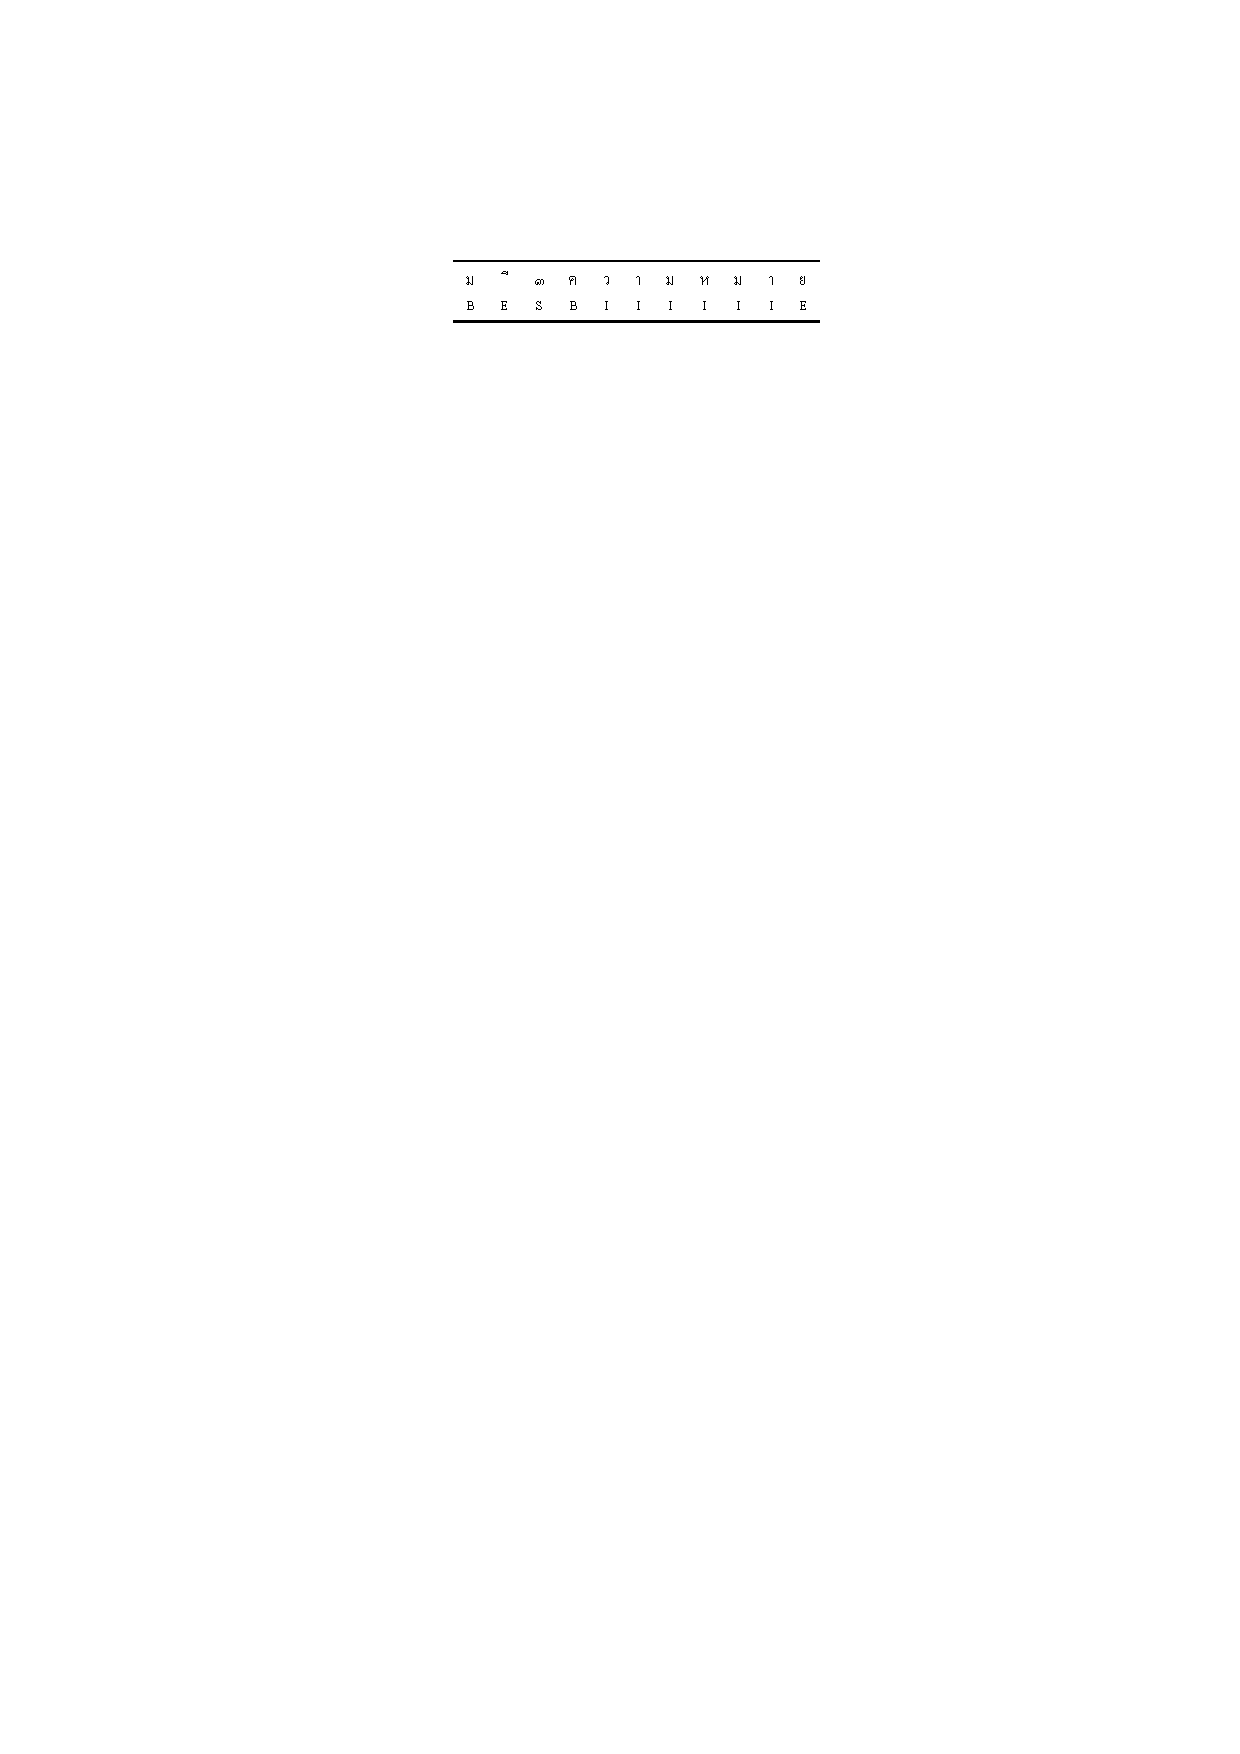
\includegraphics[width=\textwidth]{figures/fig-thbies.pdf}
    \end{subfigure}
    \hspace{\textwidth}
    \begin{subfigure}{0.24\textwidth}   
        \centering
        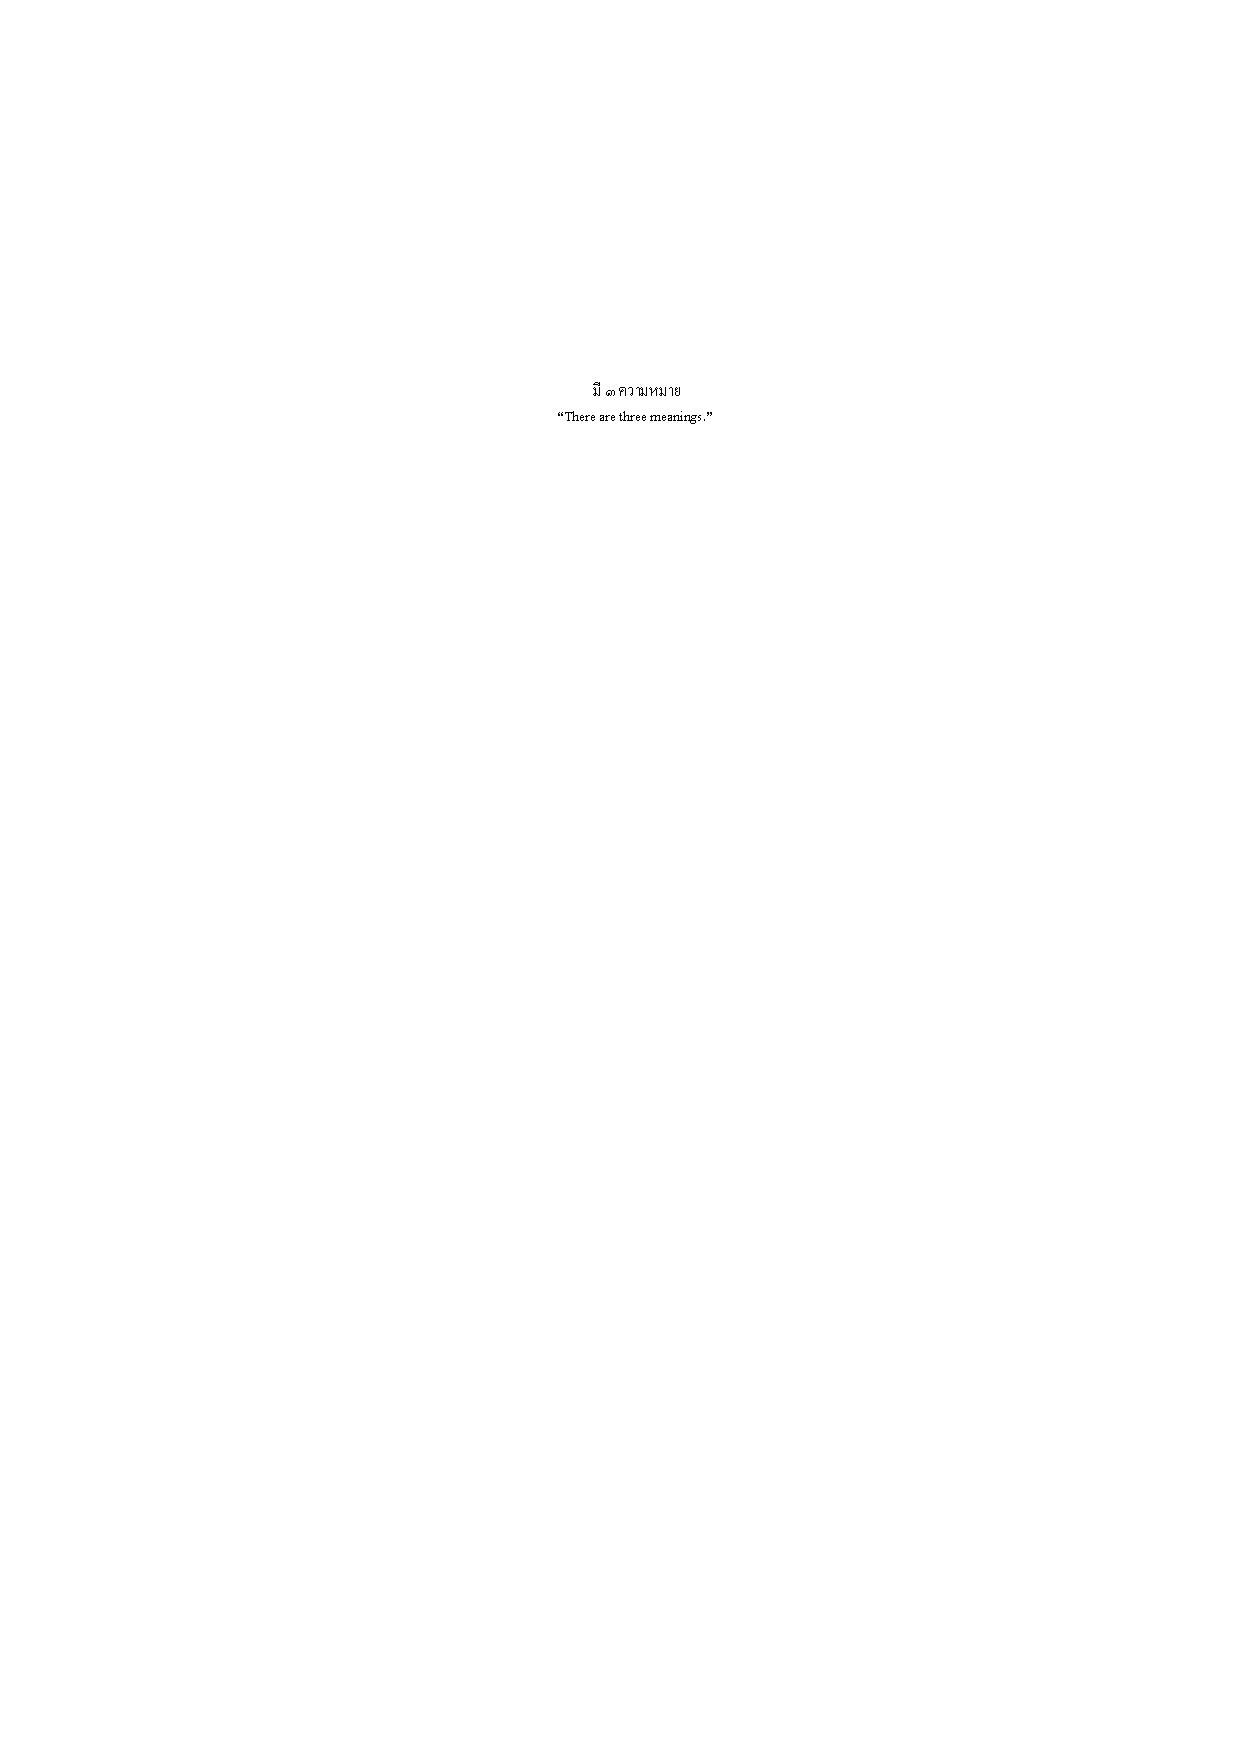
\includegraphics[width=\textwidth]{figures/fig-thbies-tran.pdf}
    \end{subfigure}
    \caption{Thai word segmentation as sequence-labeling task on BIES (beginning, inside, end, and singleton) tagging scheme.}
    \label{fig:thbies}
\end{figure}
%

Neural-network models have been applied and perform well on character-based Thai word segmentation.
%
\citeA{Jousimo2017} applied bidirectional recurrent neural networks with gated recurrent units (GRUs), while \citeA{Chormai2019} proposed an AttaCut \cite{Chormai2019},\footnote{https://github.com/PyThaiNLP/attacut} a convolutional-neural-network (CNN)-based model that mainly provides faster and more accurate word inferring motivated by DeepCut \cite{Kittinaradorn2019}.
%
% See Appendix~\ref{appx:thai-wordseg} for more details.
%
Despite the fact that neural-network models with linguistic knowledge can perform almost perfectly, adapting models with pre-trained neural networks, such as word vectors and language models, is still useful \cite{Shao2018,yan-etal-2020-bert}.
%

In spite of that a pre-trained model (PTM) such as BERT \cite{devlin-etal-2019-bert} has also been successfully applied for word segmentation mostly on Chinese datasets \cite{yang-etal-2019-bert,qiu-etal-2020-concise,ke-etal-2020-unified,huang-etal-2020-towards,ke-etal-2021-pre}, only \citeA{seeha-etal-2020-thailmcut} proposed a transfer-learning approach for Thai word segmentation by pre-training language model on the basis of character-level for character-based word segmentation. 
%
Although it exhibited state-of-the-art performance regarding Thai, it merely uses characters and does not use other information such as word and subword \cite{sennrich-etal-2016-neural,kudo-2018-subword}.
%
However, relying on the transfer-learning method can interact only input and output layers of the models, as known as black boxes, which is considered as its limitation \cite{limkonchotiwat-etal-2020-domain}. 
%
\citeA{limkonchotiwat-etal-2020-domain,limkonchotiwat-etal-2021-handling} proposed alternative approaches to particularly focus on domain-dependent word segmentation to lessen the black box limitation in the transfer learning.
%
Their works could obtain comparable results as the transfer learning method.
%

Additional linguistic-knowledge other than a character sequence, e.g., word, subword, and Thai character clusters (CCs) \cite{Theeramunkong2000} has also been successfully used for word segmentation and downstream tasks \cite{Sutantayawalee2015,Lapjaturapit2018,Nararatwong2018,yang-etal-2019-subword,li-etal-2019-word-segmentation}.
%
Furthermore, an attention mechanism \cite{Bahdanau2015} has been effectively applied to various downstream tasks, particularly a character-based sequence-labeling task that exploit more than one linguistic knowledge \cite{higashiyama-etal-2019-incorporating,tian-etal-2020-joint}.
%

To exploit multiple linguistic-knowledge, we propose a character-based Thai word-segmentation model with multiple attentions that jointly uses corresponding words, CCs, and subwords.
%
Our model is based on the bidirectional long short-term memory with conditional random field (BiLSTM-CRF) architecture, which is the baseline model for this study, because it has been successfully applied in sequence-labeling tasks for Thai and other languages \cite{Jousimo2017,Nararatwong2018,higashiyama-etal-2019-incorporating,seeha-etal-2020-thailmcut,tian-etal-2020-joint}.

%
Furthermore, Transformer-based PTM has not been incorporated in Thai word segmentation.
%
Thus, we additionally expand potential of using a pre-trained model, particularly Transformer-based PTM, in Thai word segmentation by applying BERT into our model.
%
To our best knowledge, this work is the first to adopts PTM in Thai word segmentation. 

Our contributions are as follows:
%
\begin{itemize}
    \setlength\itemsep{0.01em}
    \item We use word, CC, and subword with multiple attentions to estimate the relationships of characters in character-based Thai word segmentation.
    \item We conduct experiment for showing the validity of using CC over subword units in terms of segmentation performance and a segmentation result that does not violate Thai writing system.
    \item Our model shows improvement over the baseline model and outperforms previous works in Thai word segmentation.
    \item Our proposed model outperforms recent works that focus domain-dependent word segmentation on Thai domain-dependent datasets.
    \item We incorporate Multilingual BERT into character-based Thai word segmentation, and conduct a comparison between our BiLSTM-based model and BERT-based model. Moreover, we found that most of BERT-incorporated model could not outperform our proposed BiLSTM-based model.
    \item Our code is publicly available.\footnote{\url{https://github.com/tchayintr/thwcc-attn}}
\end{itemize}

\section{Related Work}
\subsection{Thai Word Segmentation Revisited}

In the early stage of Thai word segmentation, dictionary-based learning techniques had been used along with machine-learning techniques, for instance, Markov models \cite{Kawtrakul1997}, decision trees \cite{Sornlertlamvanich2000,Theeramunkong2001}, and CRFs \cite{Haruechaiyasak2008}.
%
CRFs have been shown to be particularly suitable for Thai sequence-labeling tasks \cite{Kruengkrai2006,Haruechaiyasak2009,Kruengkrai2009,Nararatwong2018}.
%

In parallel with CRFs, neural-network models, e.g., CNNs \cite{Kittinaradorn2019,Chormai2019}, LSTM \cite{Treeratpituk2017},\footnote{https://github.com/pucktada/cutkum} and BiLSTM \cite{Jousimo2017}, have been applied and performed excellently for character-based Thai word segmentation.
%
Using additional knowledge, such as CC \cite{Lapjaturapit2018,Nararatwong2018}, transfer learning \cite{seeha-etal-2020-thailmcut}, and stacking ensemble \cite{limkonchotiwat-etal-2020-domain,limkonchotiwat-etal-2021-handling}, along with neural-network models could improve performance.
%

\subsection{Character Clusters in Thai Word Segmentation}
Compared with English, the Thai language has various types of characters, i.e., consonants, vowels, tones, and special characters.
%
A word can be formed from a combination of these characters.
%
Thai also has unique linguistic phenomena, for example, some sequential characters tend to be indivisible units.
%
Thus, \citeA{Theeramunkong2000} introduced the concept of a CC, which is a set of predefined rules for an indivisible unit on the basis of the Thai writing system.
%

A CC is smaller than a word but larger than a character.
%
This concept is roughly comparable to a subword unit that is also in the middle of a character and word in terms of length. 
%
Using subword units, as well as CCs \cite{Theeramunkong2004,Sutantayawalee2015,Lapjaturapit2018,Nararatwong2018}, in word-segmentation tasks could yield good segmentation performance \cite{yang-etal-2019-subword,li-etal-2019-word-segmentation}.
%
However, decomposing subword units from words requires specific settings such as Byte Pair Encoding (BPE), while CCs do not require any additional settings.
%

A CC helps avoid segmenting that might violate a writing system \cite{Limcharoen2009}, while subword units will likely not thoroughly exploit morphology \cite{provilkov-etal-2020-bpe}, which could generate noise and weaken segmentation performance. 
%
This generally makes CCs smaller than subword units, as shown in Figure~\ref{fig:tccsub}, which enables a sample-comparison of segmentation results from coarse to fine (top-down) information.
%
\begin{figure}
    \centering
    \begin{subfigure}{0.49\textwidth}
        \centering
        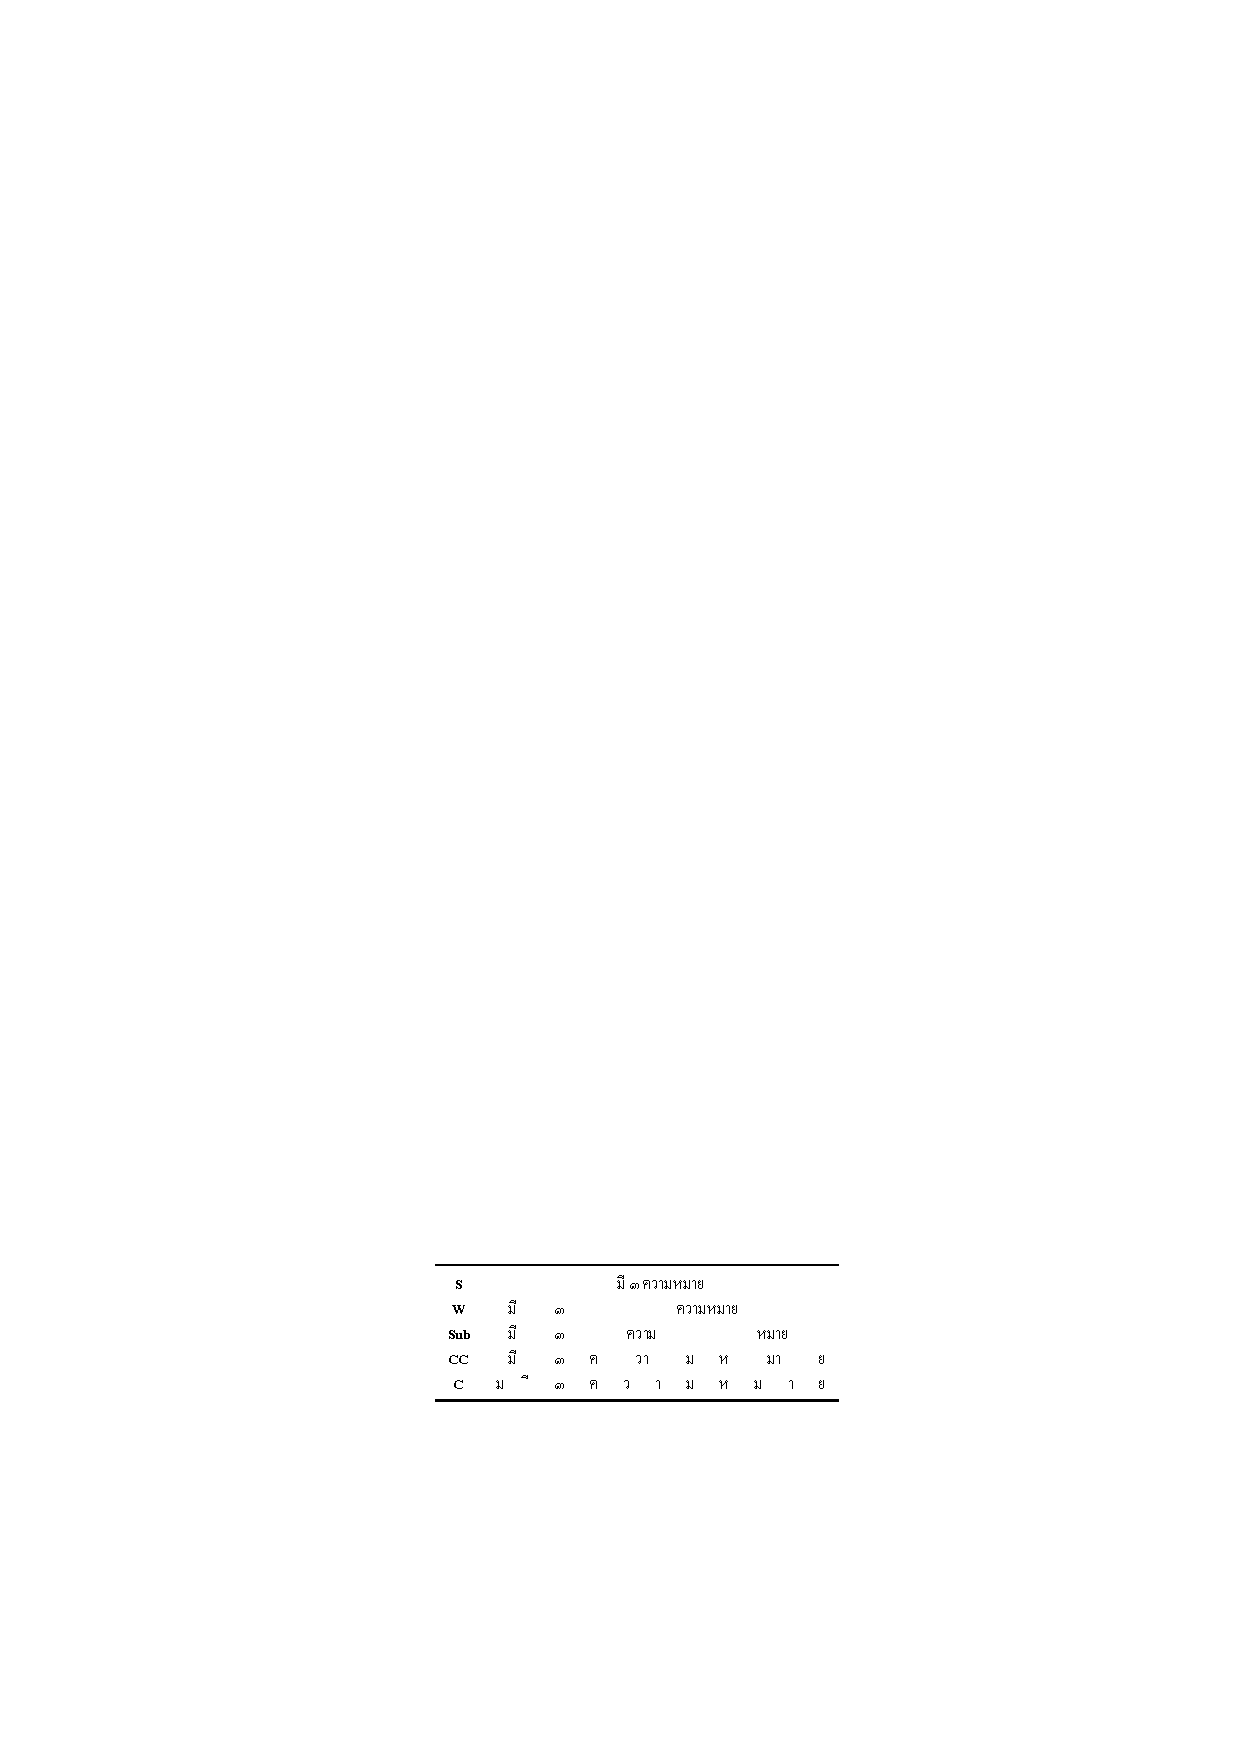
\includegraphics[width=\textwidth]{figures/fig-tccsub.pdf}
    \end{subfigure}
    \hspace{\textwidth}
    \begin{subfigure}{0.24\textwidth}
        \centering
        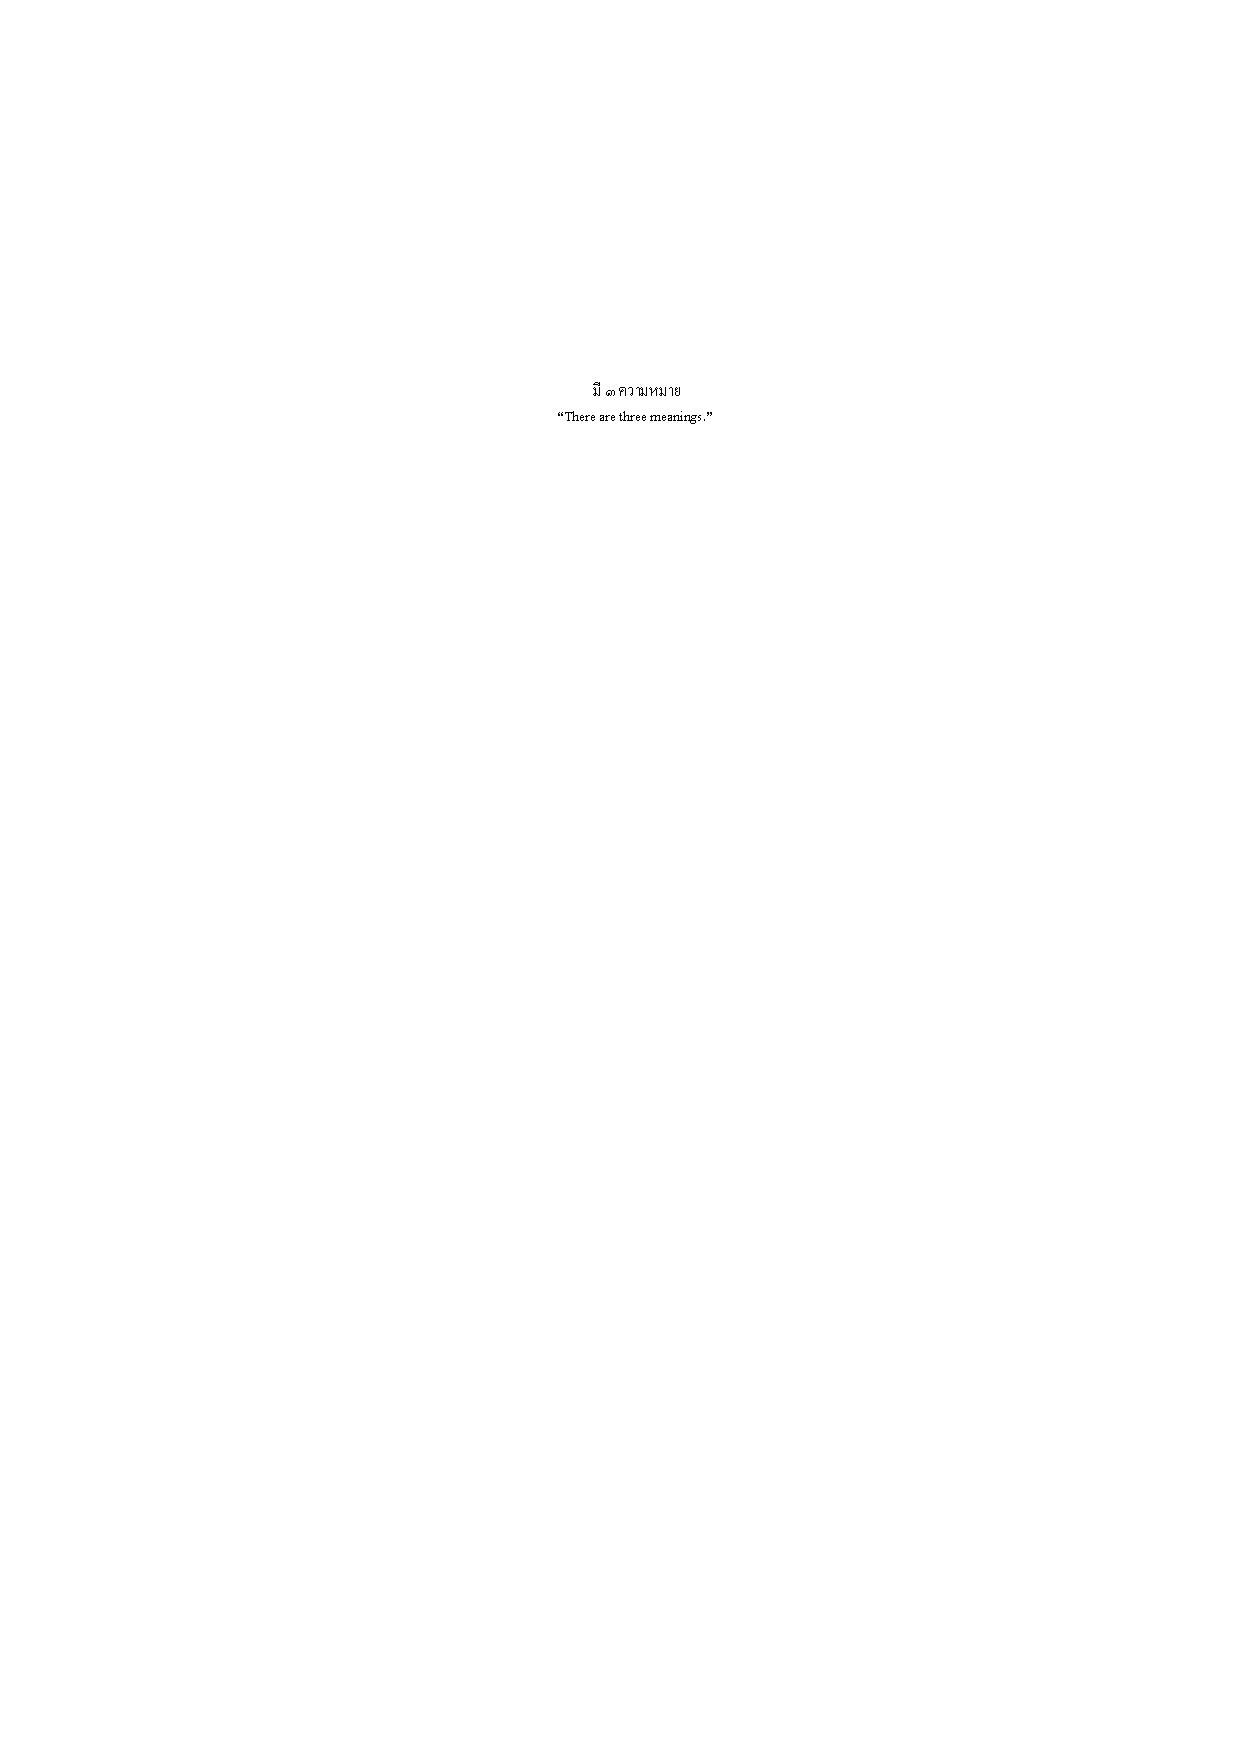
\includegraphics[width=\textwidth]{figures/fig-thbies-tran.pdf}
    \end{subfigure}
    \caption{Comparison of segmentation results. S, W, Sub, CC, and C indicate segmentation levels of sentence, word, subword, character cluster, and character, respectively.}
    \label{fig:tccsub}
\end{figure}

\subsection{Pre-trained models in Thai Word Segmentation}
Recent research works show that pre-trained models are useful for many downstream tasks, particularly Chinese Word Segmentation (CWS) \cite{yang-etal-2019-bert,qiu-etal-2020-concise,ke-etal-2020-unified,huang-etal-2020-towards,ke-etal-2021-pre}.
%
\citeA{yang-etal-2019-bert} adopted a multi-layer Bidirectional Encoder Representation from Transformers (BERT) to subword-based CWS.
%
Comparing with several neural models i.e., CNNs and BiLSTM, their work could yield better segmentation performance.
%

To our best knowledge, only \citeA{seeha-etal-2020-thailmcut} that applies PTM to Thai word segmentation. 
%
They pre-trained character-based Language Model with BiLSTM architecture and then transferred its parameters for fine-tuning character-based word segmentation afterwards. 
%
This approach set state-of-the-art performance on BEST2010 dataset,\footnote{\url{https://thailang.nectec.or.th}} which is the most well-known Thai dataset for evaluating Thai word segmentation.

\subsection{Attention Mechanism}
An attention mechanism was initially proposed by \citeA{Bahdanau2015} for neural machine translation focusing on proper parts in sentences, particularly long sentences. 
%
Basically, the attention mechanism estimates attention vectors between source and target states.
%
It has been successfully applied to downstream tasks, including machine translation \cite{luong-etal-2015-effective,Vaswani2017}, constituency parsing \cite{kitaev-klein-2018-constituency}, and sequence-labeling \cite{higashiyama-etal-2019-incorporating,tian-etal-2020-joint-chinese}.
%

\section{Approach}
Incorporating candidate words with an attention mechanism into the character-based BiLSTM-CRF architecture, as shown in Figure~\ref{fig:base-model}, could yield superb segmentation performance \cite{higashiyama-etal-2019-incorporating}.
%
An attention mechanism has the advantage of being flexible for use with additional linguistic knowledge such as CCs and subword units.
%
Thus, we use the concept of CC with an attention mechanism in character-based word segmentation, as shown in Figure \ref{fig:main-model}, by extending the BiLSTM-CRF architecture with word attention from \citeA{higashiyama-etal-2019-incorporating}.

\begin{figure}[ht]
    \centering
    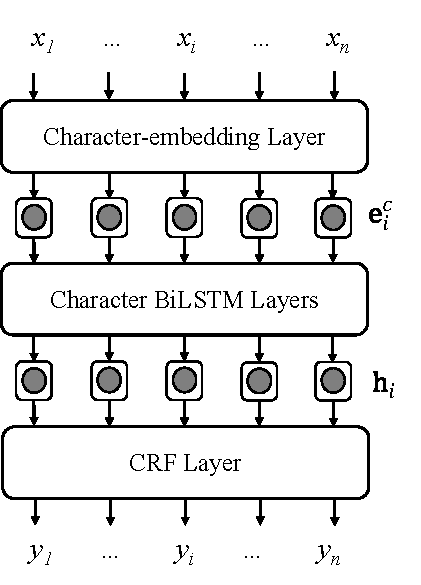
\includegraphics[width=0.3\textwidth]{figures/fig-base-model.pdf}
    \caption{Character-based BiLSTM-CRF architecture as our Baseline where $x$ and $y$ represent each character from an input sequence and a predicted label for each character, respectively. $\textbf{e}^{c}$. indicates an embedding representation for each character, and $\textbf{h}$ presents BiLSTM-encoded representation for each character.}
    \label{fig:base-model}
\end{figure}
%
Our model estimates \textit{CC-integrated character vectors} ${\textbf{z}}$ are incorporated on top of \textit{word-integrated character vectors} ${\textbf{g}}$, which are almost identical in architecture.
%
We discuss the major components of our model, i.e., the character-embedding layer, word- and CC-embedding layers, BiLSTM layers for character representation, attention integrations with the BiLSTM layers for integrated representations, CRF layer, and optional BERT layers.
%
\begin{figure}[ht]
    \centering
    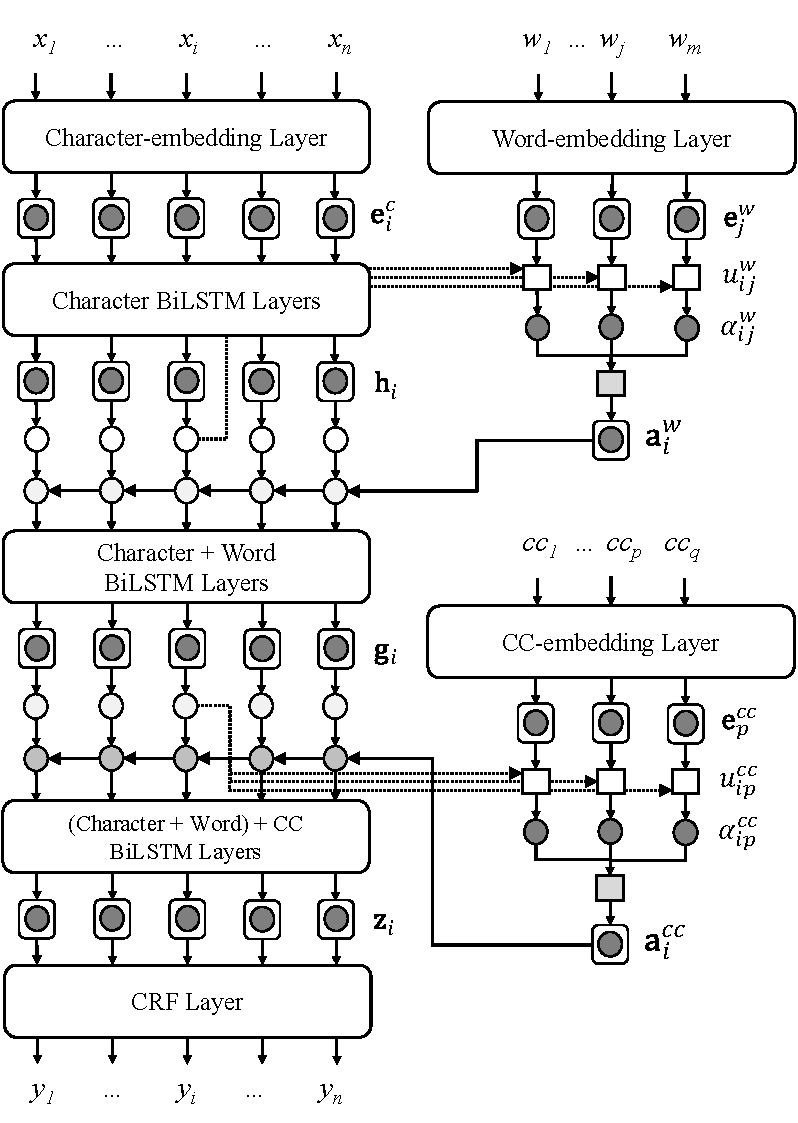
\includegraphics[width=0.58\textwidth]{figures/fig-main-model.pdf}
    \caption{Our model integrating word and CC attentions into character-based BiLSTM-CRF architecture.}
    \label{fig:main-model}
\end{figure}
%

\subsection{Character-embedding Layer}
Given a sentence $s$ with $n$ characters that can be represented as $x_{1:n} \equiv (x_1, x_2, \dots, x_n)$, each character $x_{i} \in x_{1:n}$ is transformed into a character embedding $\textbf{e}_{i}^{c}$ of a $d_{c}$-dimensional vector using lookup-table operation \cite{Bengio2003,Collobert2011}.
%
The lookup table is defined as $\text{E}^{c} \in \mathbb{R}^{d_{c} \times |V_c|}$, where $d_{c}$ denotes the dimension of embeddings and $V_c$ denotes a character vocabulary.
%
% Each character embedding $\textbf{e}_{i}^{c}$ can be obtained from the corresponding column in the lookup table $\text{E}_{1:n}^{c}$.

\subsection{Word- and CC-embedding Layers}\label{section:word-cc-embed}
Using the word embedding layer as an example, let $V_{w}$ be a word vocabulary.
%
Given the character sequence $x_{1:n}$, words are searched on the basis of $V_{w}$ within a maximum word length $K$ of the character subsequence. 
% 
A candidate word list $\mathcal{W}_{x}$ $\equiv (w_{1}, \dots, w_{m})$ of size $K$ with $m$ candidate words is then obtained, as shown in Figure~\ref{fig:main-model}.
%
Each word $w_{j} \in \mathcal{W}_{x} \subseteq V_{w}$ is transformed into a word embedding $\textbf{e}^{w}$ of a $d_{w}$-dimensional vector. 
%
The word-embedding matrix is defined as $\text{E}^{w} \in \mathbb{R}^{d_{w} \times |V_{w}|}$, where $d_{w}$ denotes the dimension of embeddings.
%
This procedure is also applied to obtain a candidate CC list $\mathcal{CC}_{x}$, which is transformed into a CC-embedding layer $\textbf{e}^{cc}$ of a $d_{cc}$-dimensional vector. 
%
The CC-embedding matrix is defined as $\text{E}^{cc} \in \mathbb{R}^{d_{cc} \times |V_{cc}|}$, where $d_{cc}$ denotes the dimension of embeddings and $V_{cc}$ denotes a CC vocabulary.

\subsection{BiLSTM Layers for Character Representation}\label{section:bilstm-for-char}
The character embedding sequence $\textbf{e}_{1:n}^{c}$ is provided to the BiLSTM \cite{Hochreiter1997,Gers2000} layers to contextually acquire \textit{character context vectors} $\textbf{h}_{1:n}$.
%

A current character context vector $\textbf{h}_{i}^{l} \in \textbf{h}_{1:n}^{l}$ of the $l$-th layer BiLSTM can be computed bidirectionally:
%
\begin{equation}
    \begin{split}
        \textbf{h}^{l}_{i} &= \text{BiLSTM}(\textbf{h}^{l-1}_{1:n}, i) \\
        & \equiv \text{LSTM}_f(\textbf{h}^{l-1}_{1:n}, i) \\
        & \oplus \text{LSTM}_b(\textbf{h}^{l-1}_{n:1}, n-i+1),
    \end{split}
    \label{eq:bilstm}
\end{equation}
where $\textbf{h}^{0}_{1:n} = \textbf{e}_{1:n}^{c}$, $\text{LSTM}_{f}$ denotes forward LSTM, $\text{LSTM}_{b}$ denotes backward LSTM, $\oplus$ denotes concatenation, and $\textbf{h} \in \mathbb{R}^{2d_{r}}$ and $d_{r}$ are hyperparameters.


\subsection{Attention Integrations with BiLSTM Layers for Integrated Representations}\label{section:attn-integration}
We use two attention integrations, including word attention and CC attention, to respectively estimate a \textit{word-integrated summary vector} $\textbf{a}_{i}^{w}$ and \textit{CC-integrated summary vector} $\textbf{a}_{i}^{cc}$ for each character in the character sequence.
%
These integrations, which are equal in architecture, accordingly summarize the relationship among characters, words, and CCs.
%

We apply the composition function \textit{weight concatenation} (WCON) \cite{higashiyama-etal-2019-incorporating,higashiyama-2022-wordseg} to estimate both summary vectors. 
%.
This function produces a word-integrated summary vector on the basis of the relationship between a character and their corresponding candidate words.
%
It also can be used to implicitly produce a CC-integrated summary vector on the basis of the relationship between the character with its corresponding candidates words and candidate CCs.

Starting with word-attention integration, we estimate the word-importance score $u_{ij}^{w}$ and word-attention weight $\alpha_{ij}^{w}$ on the basis of the character context vector $\textbf{h}_{i}$ and candidate word embedding $\textbf{e}_{j}^{w}$ as
% %
\begin{equation}
    u_{ij}^{w} = \textbf{h}_i^{T}W_{a}^{w}\textbf{e}_{j}^{w},
    \label{eq:word-important}
\end{equation}
%
\begin{equation}
    \alpha_{ij}^{w} = \frac{\delta_{ij}\exp(u_{ij}^{w})}{\sum_{k=1}^{m}\delta_{ik}\exp(u_{ik}^{w})},
    \label{eq:word-attn-weight}
\end{equation}
%
where $W_{a}^{w} \in \mathbb{R}^{2d_{r} \times d_{w}}$ denotes a trainable weight matrix and $\delta_{ij} \in \{0,1\}$ indicates whether character $x_{i}$ is included in candidate word $w_{j}$.
%
The word-integrated summary vector $\textbf{a}_{i}^{w}$ for character $x_{i}$ can be calculated as
%
\begin{equation}
    \textbf{a}_{i}^{w} = \text{WCON}^{w}(x_{i}, \{w_{j}\}_{j=1}^{m}) {=} \bigoplus_{l=1}^{L^{w}}\alpha_{i,i_{l}}^{w}\textbf{e}_{i_{l}}^{w},
    \label{eq:wcon}
\end{equation}
%
where \{$w_{j}$\} = $\mathcal{W}_{x}$. 
%
Let $K^{w}$ be the maximum word length, $L^{w} = \sum_{k=1}^{K^{w }}k$, $\bigoplus$ denote concatenation, and $i_{l}$ is the corresponding index of candidate word list $\mathcal{W}_{x}$ for character $x_{i}$ that is $\{w^{\prime}_{1},\dots,w^{\prime}_{L^{w}}\} \equiv \bigcup_{k=1}^{K^{w}}\bigcup_{s=-k+1}^{0}\{x_{i+s:i+s+k-1}\}$.
%
Note that a zero vector is applied to Equation \ref{eq:wcon} when $w^{\prime}_{l} \notin V_{w}$.
%

For instance, to compose the list of words $w^{\prime}_{4}$ containing a character $x_{4}$ for estimating the word-importance score $u^{w}_{4,j}$, the word-attention weight $\alpha^{w}_{4,j}$, and the summary vector $\textbf{a}^{w}_{4}$, let the candidate words list $\mathcal{W}_{x} = \{w_{1},\dots,w_{8}\}$, maximum word length $K^{w} = 4$, and $L^{w} = \sum_{k=1}^{K^{w }}k = 10$, the procedure can be performed as follows:
%
\begin{equation}
    \begin{split}
        w^{\prime}_{4} &= \bigcup_{k=1}^{4}\bigcup_{s=-k+1}^{0} \{x_{4+s:4+s+k-1}\} \\
        & = \{x_{4:4},x_{4:3},x_{4:5},x_{2:4},x_{3:5},x_{4:6},x_{1:4},x_{2:5},x_{3:6},x_{4:7}\}.
    \end{split}
    \label{eq:wcon-x4}
\end{equation}
where the words $x \in w^{\prime}_{4}$ containing in train vocabulary will be used.
%

We then use the BiLSTM layers for transforming the word-integrated summary vectors $\textbf{a}^{w}$ into word-integrated character vectors $\textbf{g}$. 
%
The operation of word-integrated character vector $\textbf{g}_{i}$ is computed using the BiLSTM layers on the basis of word-integrated summary vector $\textbf{a}_{i}^{w}$ with its corresponding character context vector $\textbf{h}_{i}$ as 
%
\begin{equation}
    \textbf{g}_{i} = \text{BiLSTM}(\textbf{h}_{i}\oplus\textbf{a}_{i}^{w}).
    \label{eq:wcon-concat}
\end{equation}
%

However, the candidate CCs that correspond to the character are used on top of $\textbf{g}_{i}$ as
%

\begin{gather}
    u_{ip}^{cc} = \textbf{g}_i^{T}W_{a}^{cc}\textbf{e}_{p}^{cc}, \label{eq:ccwcon-score}\\
    \alpha_{ip}^{cc} = \frac{\delta_{ip}\exp(u_{ip}^{cc})}{\sum_{k=1}^{q}\delta_{ik}\exp(u_{ik}^{cc})},
\end{gather}
%
where $W_{a}^{cc} \in \mathbb{R}^{4d_{r} \times d_{cc}}$ denotes a trainable weight matrix and $\delta_{ip} \in \{0,1\}$ indicates whether character $x_{i}$ is included in the candidate CC $cc_{p}$.
%
The CC-integrated summary vector $\textbf{a}_{i}^{cc}$ for character $x_{i}$ can be calculated as
\begin{equation}
    \textbf{a}_{i}^{cc} = \text{WCON}^{cc}(x_{i}, \{cc_{p}\}_{p=1}^{q}) {=} \bigoplus_{l=1}^{L^{cc}}\alpha_{i,i_{l}}^{cc}\textbf{e}_{i_{l}}^{cc},
    \label{eq:ccwcon}
\end{equation}
%
where \{$cc_{p}$\} = $\mathcal{CC}_{x}$. 
%
Let $K^{cc}$ is the maximum CC length, $L^{cc} = \sum_{k=1}^{K^{cc}}k$, and $i_{l}$ is the corresponding index of potential CC list $\mathcal{CC}_{x}$ for character $x_{i}$, which is represented by $\{cc^{\prime}_{1},\dots,cc^{\prime}_{L^{cc}}\} \equiv \bigcup_{k=1}^{K^{cc}}\bigcup_{s=-k+1}^{0}\{x_{i+s:i+s+k-1}\}$.
%
A zero vector is applied to Equation \ref{eq:ccwcon} when $cc^{\prime}_{l} \notin \mathcal{V}_{cc}$.

Next, we use additional BiLSTM layers to transform the CC-integrated summary vectors $\textbf{a}^{cc}$ into CC-integrated character vectors $\textbf{z}$ on the basis of a cluster-integrated summary vector $\textbf{a}_{i}^{cc}$ and its corresponding word-integrated character vector $\textbf{g}_{i}$ as 
%
\begin{equation}
    \textbf{z}_{i} = \text{BiLSTM}(\textbf{g}_{i}\oplus\textbf{a}_{i}^{cc}).
    \label{eq:ccwcon-concat}
\end{equation}
%
A CRF is finally used to estimate the probability of the optimal label sequences $y$.

\subsection{CRF Layer}
A CRF \cite{Lafferty2001} along with explicitly considering the correlations between adjacent labels has been successfully applied for sequence-labeling-related tasks \cite{Collobert2011}.
%
Let $A \in \mathbb{R}^{|T| \times |T|}$ be a transition matrix for correlations between adjacent labels, where $T$ denotes a set of all possible label sequences, for instance, $T = \{B, I, E, S\}$.
%
The CC-integrated character vector $\textbf{z}_{i}$ is transformed into an un-normalized label score $\textbf{s}_{i}$ of the $|T|$-dimensional vector for character $x_i$ as
%
\begin{equation}
    \textbf{s}_i = W_{s}\textbf{z}_{i} + \textbf{b}_{s},
\end{equation}
where $W_{s} \in \mathbb{R}^{|T| \times 4d_{r}}$ denotes a trainable weight matrix, and $\textbf{b}_{s} \in \mathbb{R}^{|T|}$ denotes a trainable bias. 
%
Given the input sequence $x_{1:n}$, the corresponding scores for the label sequence $y_{1:n}$ are computed on the basis of transition matrix $A$ and the segmentation label scores $\textbf{s}$ as follows:
\begin{equation}
    \text{score}(x, y) = \sum_{i=1}^{n}(A_{y_{i-1},{y_i}} + \textbf{s}_i[y_{i}]).
\end{equation}
%
The probability of the label sequence can then be obtained as
%
\begin{equation}
    P(y|x) = \frac{\text{score}(x,y)}{\sum_{y' \in T^{n}}\text{score}(x,y')}.
\end{equation}
%
We can obtain the optimal label sequence $y^{\star}$ by maximizing the sentence score with the Viterbi algorithm:
%
\begin{equation}
    y^{\star} = \text{argmax}_{y \in T^{n}}\text{score}(x,y).
\end{equation}
%
The loss function $\mathcal{L}$ is minimized by back propagation during the training process:
%
\begin{equation}
    \mathcal{L}(x,y) = - \log P(y|x).
\end{equation}

\subsection{BERT Layers}
In this work, we use BERT layers for comparing with BiLSTM-based models. 
%
$\text{BERT}_{base}$ layer\footnote{https://huggingface.co/bert-base-multilingual-cased} is used to extract three types of representation, including contextual-character-, word-, and CC-representation.
%
Concretely, we replace the BiLSTM layers for character representation in Section \ref{section:bilstm-for-char} with BERT-encoder layer to compute the \textit{character context vectors} $\textbf{h}_{1:n}$ that can be represented in \ref{fig:bert-model}. 
%
The current character context vector $\textbf{h}_{i}$ can be computed: 
\begin{equation}
    \textbf{h}_{i}^{0} = {\textbf{e}^{c}}_{i} + {\textbf{e}^{p}_{i}},
\end{equation}

\begin{equation}
    \textbf{h}_{i}^{l} = \text{Transformer}(\textbf{h}_{i}^{l-1}),
\end{equation}
%
where $l = \{1, 2, \dots, L\}$, which is the number of transformer layers \cite{Vaswani2017}. $\textbf{e}^{c}$ is the embedding obtained from the BERT-embedding layer while $\textbf{e}^{p}$ is the positional embedding.
%
Because we adopt $\text{BERT}_{base}$, $L=12$. $e^{c} \in \mathbb{R}^{d_{c} \times |V_{\text{BERT}}|}$, where $d_{c} = 768$, and $V_{\text{BERT}}$ denotes the vocabulary in $\text{BERT}_{base}$.
%
For the word- and CC-representation, which can be referred in \ref{section:word-cc-embed}, we straightforwardly obtain their representations from the embedding layer of BERT. 
%
In other words, word- and cc-embedding layer (as well as subword-embedding layer) are replaced with BERT-embedding layer.
%
By using the BERT embedding layers, the word- and CC-embedding matrices are defined as $\text{E}^{w} \in \mathbb{R}^{d_{w} \times |V_{\text{BERT}}|}$ and $\text{E}^{cc} \in \mathbb{R}^{d_{cc} \times |V_{\text{BERT}}|}$, where $d_{w}=768$, $d_{cc}=768$.
%
Finally, the BERT-pooler layer and CRF layer are used to conditionally project the BERT representations from its encoder layers into the optimal label sequences $y^{\star}$.

\begin{figure}[ht]
    \centering
    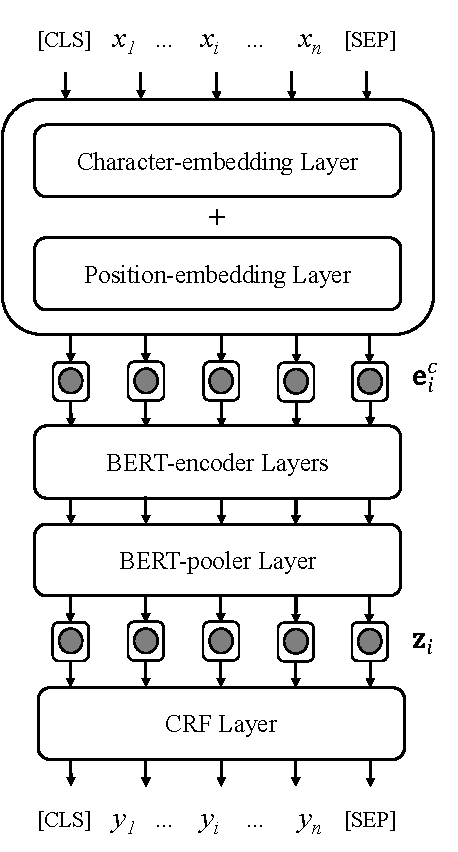
\includegraphics[width=0.35\textwidth]{figures/fig-bert-ext-model.pdf}
    \caption{Character-based word-segmentation model incorporated with BERT pre-trained model.}
    \label{fig:bert-model}
\end{figure}

\section{Experiment}
\subsection{Datasets} 
%
We trained and evaluated several versions of our model on three datasets, BEST2010, TNHC,\footnote{\url{https://attapol.github.io/tlc}} and VISTEC.\footnote{\url{https://github.com/mrpeerat/OSKut/tree/main/VISTEC-TP-TH-2021}}
%
BEST2010 corpus consists of four different domains of textual document, including article, encyclopedia, news, and novel.
%
It has been used to mainly evaluate Thai word segmentation models.
%
TNHC and VISTEC are a collection of Thai classical literature and a social media dataset for Thai text processing, respectively.
%
The latter two datasets have been recently used for evaluating in domain-dependent word segmentation.
%
We randomly split the BEST2010 corpus into three sets:\footnote{\url{https://resources.aiat.or.th/thwcc-attn/datasets}} 80\% for a training, 10\% for a validation, and 10\% for a test.
%
For TNHC and VISTEC, we followed the same data splits as in previous work \cite{limkonchotiwat-etal-2020-domain,limkonchotiwat-etal-2021-handling}.
%
The data lengths for all datasets are listed in Table~\ref{tab:dataset}.
%
\begin{table}
\centering
\scalebox{1.0}{
\begin{tabular}{llcccc}
\hline
\textbf{Dataset}          & \textbf{Set} & \textbf{$|$S$|$} & \textbf{$|$W$|$} & \textbf{$|$V$|$} & \textbf{$|$Ch$|$} \\ \hline
\multirow{3}{*}{BEST2010} & Train        & 119K             & 4M               & 72.9K            & 16M               \\
                          & Valid        & 14.9K            & 501.4K           & 23K              & 1.9M              \\
                          & Test         & 14.9K            & 500.4K           & 23K              & 1.9M              \\ \hline
\multirow{3}{*}{TNHC}     & Train        & 12.7K            & 0.3M             & 16.8K            & 1.3M              \\
                          & Valid        & 1.4K             & 47.2K            & 5.3K             & 0.1M              \\
                          & Test         & 4.4K             & 125K             & 9.2K             & 0.4M              \\ \hline
\multirow{3}{*}{VISTEC}   & Train        & 36K              & 2.4M             & 98.5K            & 9.5M              \\
                          & Valid        & 4K               & 270K             & 23.7K            & 1.1M              \\
                          & Test         & 10K              & 677.4K           & 42.9K            & 2.6M              \\ \hline
\end{tabular}}
\caption{Data size, including the number of sentences (S), words (W), vocabulary (V), and characters (Ch).}
\label{tab:dataset}
\end{table}

\subsection{Subword-unit Integration}
Although subword units have been successfully applied to the word-segmentation task, they might generate noise that decreases segmentation performance when the word dictionary already exists.
%
Therefore, we conducted a comparison of using either subword units or CCs due to their similarity on the different versions of our proposed model. 
%
Let $V_{sw}$ be a subword vocabulary decomposed from the dataset.
%
We simply replace the CC vocabulary $V_{cc}$ with the decomposed subword vocabulary $V_{sw}$.
%
Thus, a candidate subwords list  $\mathcal{SW}_{x}$ can be acquired and used for the subword-attention integration by applying Equations \ref{eq:ccwcon-score} and \ref{eq:ccwcon}.

\subsection{Integration Order of Word and CC Attention(s)}
Considering the flexibility of attention integration, the integration order in our model can be switched.
%
For instance, our model executes CC-attention integration to estimate the relationship between characters and CCs before word-attention integration.
%
This might affect segmentation performance because each integration provides different knowledge.
%
Thus, we implemented a swapped version of our model (Swap) that switches the integration order for comparing the segmentation performance.

\subsection{Pre-trained Model Integration}
Fine-tuning a pre-trained model for word segmentation models has been been proved to be effective.
%
Thus, we conducted a character-based Thai word segmentation with pre-trained model, which is shown in Figure \ref{fig:bert-model}, by simply replacing the character BiLSTM layers in Figure \ref{fig:base-model} with BERT layers.
%
We chose Multilingual BERT\footnote{https://huggingface.co/bert-base-multilingual-cased} for our experiment due to its originality and accessibility. 
%
Furthermore, we also applied this approach to the baseline model and our proposed model, where word, CCs, or subword units are used, for model comparison.
%

In our experiment, concretely, each character $x_{i}$ is transformed into BERT-token id.
%
Thereafter, each token id is encoded with BERT encoder to obtain a character BERT-representation.
%
Candidate word $w_{j}$, and either candidate CC $cc_{p}$ or candidate subword unit $sw_{p}$ obtained from Section \ref{section:attn-integration} are transformed into BERT-token id.
%
Unlike the character BERT-representation, such candidate units are encoded into word-, CC-, subword-BERT-representation, from BERT-embedding layer directly.
%
The character BERT-representation along with corresponding word BERT-representation and either CC BERT-representation or subword BERT-representation are, used to estimate the importance scores $u$ and the attention weights $\alpha$ in Section \ref{section:attn-integration}.
%
Note that BERT tokenizer are not used to tokenize the sentence $s$ into subword units.
%
Thus, the candidate word, CC, and subword unit, can be unknown token (UNK), in other words, it depends on pre-trained model and is used as well as an approach to construct subword units in this experiment.
%

In addition, we included special tokens, including CLS and SEP tokens, in training-, validation-, and test-step, as the S (single-word) label of BIES tagging scheme.
%
However, these special tokens are not counted in testing step to avoid the overestimation.

\subsection{Compared Models}
%
We evaluated the following models:

\begin{itemize}
    \setlength\itemsep{0.01em}
    \item\textbf{Baseline}:
        A character-based BiLSTM-CRF architecture as shown in Figure~\ref{fig:base-model}.
    \item\textbf{Baseline w/ Word}:
        An extension of Baseline that integrates word attention (BiLSTM-CRF with word attention) \cite{higashiyama-etal-2019-incorporating}.
    \item\textbf{Baseline w/o BiLSTM w/ BERT}:
        A character-based BERT-CRF architecture that replaces BiLSTM layers for character representation with BERT layers, as shown in \ref{fig:bert-model}.
    \item\textbf{Baseline w/ BERT w/ Word}:
        The Baseline w/ Word that replaces BiLSTM layers for character representation with BERT (BERT-BiLSTM-CRF with word attention).
    \item\textbf{OURS}:
        Our proposed model that integrates word and CC attentions (BiLSTM-CRF with word and CC attentions), as shown in Figure~\ref{fig:main-model}.
    \item\textbf{OURS w/o CC w/ Sub}:
        Our proposed model that replaces the CC with various sizes of subword units (800-12,800) (BiLSTM-CRF with word and subword attentions).
    \item\textbf{OURS w/o Word}:
        Our proposed model that removes word attention (BiLSTM-CRF with CC attention).
    \item\textbf{OURS Swap}:
        Our proposed model that swaps the order of word and CC attentions.
    \item\textbf{OURS w/o CC w/ Sub Swap}: 
        OURS w/o CC w/ Sub model that swaps the order of word and subword unit attentions.
    \item\textbf{OURS w/ BERT}:
        Our proposed model that integrates word and CC attentions, and replaces BiLSTM layers for character representation with BERT (BERT-BiLSTM-CRF with word and CC attentions).
    \item\textbf{OURS w/ BERT w/o CC w/ Sub}:
        Our proposed model that integrates word and subword unit attentions, and replaces BiLSTM layers for character representation with BERT (BERT-BiLSTM-CRF with word and subword attentions).
    \item\textbf{Others}: Reproduced Thai non-neural/neural word-segmentation models, including well-known models, the state-of-the-art Thai word-segmentation model \cite{seeha-etal-2020-thailmcut}, and recent domain-adaptation models \cite{limkonchotiwat-etal-2020-domain,limkonchotiwat-etal-2021-handling}.
\end{itemize}

We used CCs with publicly available libraries, including \citeA{pythainlp} and TCCSEG,\footnote{\url{https://github.com/tchayintr/tccseg}} to build the CC vocabulary $V_{cc}$.
%
To generate the subword vocabulary $V_{sw}$ for each dataset, we decomposed raw sentences from train set  into various sizes of subword units using byte-pair encoding \cite{sennrich-etal-2016-neural} implemented by SentencePiece \cite{kudo-richardson-2018-sentencepiece}. Note that the generated subword vocabulary for each dataset is not shared among the experimental datasets.

%
% We utilized the common hyperparameters for training our proposed modeals, as in Appendix. 
We used the common hyperparameters for training the different versions of our proposed model (hereafter, our models), as shown in Table~\ref{tab:hyp}.
% We utilized the common hyperparameters for training our proposed models, as in Appendix~\ref{appx:hyp}. 
%
Dropout \cite{Srivastava2014} was applied to the BiLSTM layers to avoid overfitting as well as non-recurrent layers \cite{Zaremba2015}.
%
We also optimized the model parameters using the Adam optimizer \cite{Kingma2015}.
%
We trained our models up to 20 epochs and chose the best one on the basis of the validation process involving word-level evaluation (CoNLL\footnote{\url{https://github.com/spyysalo/conlleval.py}}).
%

We evaluated our models on the test data by using three evaluation metrics, i.e., word-level evaluation (CoNLL-format), BIES tagging scheme (character-level evaluation), and Bound (boundary-level evaluation) \cite{seeha-etal-2020-thailmcut}.
%
% We used word-level, BIES tagging schemes, and the boundary-level evaluation to evaluate the segmentation performance in our experiments.
% %
Moreover, we additionally used binary-character-level evaluation similar to \citeA{limkonchotiwat-etal-2020-domain,limkonchotiwat-etal-2021-handling} for comparing our model with the recent Thai domain-adaptation word segmentation works.
%
% The boundary-level evaluations are defined as
% \begin{gather*}
%     \text{P} = \frac{\text{\# correct predicted word boundaries}}{\text{\# predicted characters as word boundaries}} \\
%     \text{R} = \frac{\text{\# correct predicted word boundaries}}{\text{\# hypothesis word boundaries}} \\
%     \text{F$_{1}$} = \text{2} \times \frac{\text{P} \times \text{R}}{\text{P} + \text{R}},
% \end{gather*}
% %
% where P, R, and F$_{1}$ denote the precision, recall, and F$_{1}$ score, respectively.
%
Note that our F$_{1}$ scores are based on the micro-averaged F$_{1}$ score for all evaluation matrices.
% We evaluated our models based on the test data by three evaluation metrics (Appendix~\ref{appx:eval-metrics}), including CoNLL\footnote{\url{https://github.com/spyysalo/conlleval.py}}, Boundary-level \cite{seeha-etal-2020-thailmcut}, and BIES tagging schemes that averages micro-averaged F$_{1}$ scores for each label.
%
We conducted statistical significance tests using paired bootstrap resampling \cite{Koehn2004} on our results, particularly OURS with the Thai state-of-the-art word segmentation \cite{seeha-etal-2020-thailmcut}, OURS with Baseline w/ Word \cite{higashinaka-etal-2021-integrated}, and OURS w/o CC w/ Sub.
%  
We set the resampling size to 100,000 iterations and sample size for each resampling to 10\% of the test data.

\begin{table}
\centering
\scalebox{1.0}{
\begin{tabular}{lr}
\hline
\textbf{Parameter}             & \textbf{Value} \\ \hline
Character-embedding size       & 128            \\
BiLSTM layers                  & 2              \\
BiLSTM hidden size             & 600            \\
Mini-batch size                & 128            \\
BiLSTM Initial learning rate   & 0.001          \\
Learning rate decay            & 0.99           \\
Recurrent layer dropout rate   & 0.4            \\ \hline
Word-embedding size            & 300            \\
Word-vector dropout rate       & 0.4            \\
Maximum word (chunk) length    & 4              \\ 
BERT hidden size               & 768            \\
BERT initial learning rate     & 0.00002        \\
Maximum sequence length        & 512            \\ \hline
CC/subword-embedding size      & 300            \\
CC/subword-vector dropout rate & 0.4            \\
Maximum CC/subword length      & 0.4            \\ \hline
\end{tabular}}
\caption{Common hyperparameters for Baselines and our models (top/middle) with exclusive values for our models (bottom). CC hyperparameters can be applied to subword integration.}
\label{tab:hyp}
\end{table}



\section{Results and Discussion}
\subsection{Main Results}\label{section:main-results}

Table~\ref{tab:main-results}\footnote{We used LexTo (http://www.sansarn.com/lexto), TLTK (https://github.com/attapol/tltk), Multi-cut, and New Multi-cut (https://github.com/PyThaiNLP) to produce non-neural segmentation results} illustrates the evaluation results among the compared models on BERT2010.
%
The best of our models, i.e., OURS, achieved the state-of-the-art performance compared with all the other models.
%
From the statistical significance test results, we concluded that OURS surpasses the state-of-the-art model and the strong baseline models, i.e., Baseline w/ Word and OURS w/o CC w/ Sub.
%
Although using subword units could slightly improve its performance compared with using CCs, OURS outperformed OURS w/o CC w/ Sub on multiple runs as well as performing significantly better at p-level $< 0.05$. 
%
This indicates that CCs are more beneficial than subword units in terms of segmentation performance, moreover, unlike incorporating subword, CCs does not require hyperparameter adjustment.
%
OURS, which uses word and CC information, outperformed Baseline w/ Word, which indicates that CCs can be used to complement linguistic knowledge, particularly word information.
%
We implemented an additional model that replaces the BiLSTM layers with Transformer layers \cite{Vaswani2017} in Baseline. However, the results were noticeably lower than all other models. Note that we used the hyperparameters for the Transformer layers by referring to \citeA{Vaswani2017}.
%
In addition to the non-neural models, every model could not outperform any neural model.
%
However, as for TLTK and New Multi-Cut that incorporate with additional linguistic knowledge, i.e., Syllable and CC, show the benefits over LexTo and Multi-Cut in term of segmentation performance.
%
The results show that incorporating with Syllable obviously boosts Word-F1 score and Bound-F1 while CC could help in improving BIES-F1.

\begin{table}
\centering
\scalebox{0.78}{
\begin{tabular}{llccc}
\hline
\textbf{Model} &
  \textbf{Method} &
  \textbf{\begin{tabular}[c]{@{}c@{}}Word-F1\\ ($\sigma$)\end{tabular}} &
  \textbf{\begin{tabular}[c]{@{}c@{}}BIES-F1\\ ($\sigma$)\end{tabular}} &
  \textbf{\begin{tabular}[c]{@{}c@{}}Bound-F1\\ ($\sigma$)\end{tabular}} \\ \hline
LexTo $^\circ$$^\odot$                   & Dict w/ Longest-matching                & 67.29                     & 84.38                  & 91.32                  \\
TLTK $^\circ$$^\odot$                    & Dict w/ Maximum-collocation w/ Syllable & 74.49                     & 86.00                  & 93.01                  \\
Multi-Cut $^\circ$$^\odot$               & Dict w/ Maximum-matching                & 60.36                     & 83.34                  & 88.95                  \\
New Multi-Cut $^\circ$$^\odot$           & Dict w/ Maximum-matching w/ CC          & 68.63                     & 86.39                  & 91.81                  \\ \hdashline
\cite{Treeratpituk2017}$^\circ$          & LSTM                                    & 92.49                     & 96.53                  & 97.94                  \\
\cite{Chormai2019}$^\circ$               & CNN w/ Syllable                         & 93.79                     & 91.36                  & 98.36                  \\
\cite{Kittinaradorn2019}$^\circ$         & CNN w/ Char-type                        & 95.82                     & 98.17                  & 98.87                  \\
\cite{Lapjaturapit2018}$^\circ$          & BiLSTM w/ CC                            & 96.22                     & 98.43                  & 99.03                  \\
\cite{seeha-etal-2020-thailmcut}$^\circ$ & BiLSTM w/ Char-PTM                      & \underline{97.20}         & 98.80                  & 99.27                  \\ \hline
Baseline                                 & BiLSTM-CRF                              & 96.71 (0.120)             & 98.28 (0.117)          & 99.15 (0.023)          \\
Baseline w/ Word                         & BiLSTM-CRF w/ Word                      & \underline{97.57} (0.003) & 98.94 (0.008)          & 99.35 (0.008)          \\ \hdashline
Baseline w/o BiLSTM w/ BERT              & BERT-CRF                                & 97.18 (0.012)             & 98.77 (0.029)          & 99.24 (0.021)          \\
Baseline w/ BERT w/ Word                 & BERT-BiLSTM-CRF w/ Word                 & 96.79 (0.310)             & 98.65 (0.095)          & 99.15 (0.080)          \\ \hline
OURS                                     & BiLSTM-CRF w/ Word w/ CC                & \textbf{97.67} (0.020)    & \textbf{98.99} (0.005) & \textbf{99.38} (0.006) \\
OURS w/o CC w/ Sub                       & BiLSTM-CRF w/ Word w/ Sub               & \underline{97.60} (0.035)             & 98.96 (0.021)          & 99.35 (0.009)          \\
OURS w/o Word                            & BiLSTM-CRF w/ CC                        & 97.42 (0.020)             & 98.91 (0.012)          & 99.32 (0.007)          \\
OURS Swap                                & BiLSTM-CRF w/ Word w/ CC Swap           & 97.61 (0.010)             & 98.97 (0.012)          & 99.36 (0.008)          \\
OURS w/o CC w/ Sub Swap                  & BiLSTM-CRF w/ Word w/ Sub Swap          & 97.45 (0.041)             & 98.87 (0.046)          & 99.32 (0.024)          \\ \hdashline
OURS w/ BERT                             & BERT-BiLSTM-CRF w/ Word w/ CC           & 97.24 (0.030)             & 98.92 (0.020)          & 99.27 (0.016)          \\
OURS w/ BERT w/o CC w/ Sub               & BERT-BiLSTM-CRF w/ Word w/ Sub          & 97.11 (0.081)             & 98.76 (0.049)          & 99.23 (0.035)          \\ \hline
\end{tabular}}
\caption{Comparison among our models, baselines, and Others on BEST2010. Best score for each metric is indicated in \textbf{bold}. OURS was significantly better than state-of-the-art model Thai word segmentation model, Baseline w/ Word, and OURS w/o CC w/ Sub (\underline{underline} scores) at p-level $< 0.05$ in pairwise comparison. All models were evaluated on basis of same dataset division. The scores were obtained from mean of three runs. OURS w/o CC w/ Sub scores were reported on the basis of best validation performance among various subword vocabulary sizes. $\circ$ and $\odot$ indicate reproduced Thai word-segmentation models, and non-neural Thai word-segmentation models, respectively. $\sigma$ represents Population standard deviation.}
\label{tab:main-results}
\end{table}

\begin{table}
\centering
\scalebox{0.83}{
\begin{tabular}{llccccc}
\hline
\textbf{Model} &
  \textbf{Method} &
  \textbf{Word} &
  \textbf{CC} &
  \textbf{Sub} &
  \textbf{LSTM} &
  \textbf{PTM} \\ \hline
LexTo $^\circ$$^\odot$ &
  Dict w/ Longest-matching &
  \multicolumn{1}{l}{\checkmark} &
  \multicolumn{1}{l}{} &
  \multicolumn{1}{l}{} &
  \multicolumn{1}{l}{} &
  \multicolumn{1}{l}{} \\
TLTK $^\circ$$^\odot$ &
  Dict w/ Maximum-collocation w/ Syllable &
  \multicolumn{1}{l}{\checkmark} &
  \multicolumn{1}{l}{} &
  \multicolumn{1}{l}{} &
  \multicolumn{1}{l}{} &
  \multicolumn{1}{l}{} \\
Multi-Cut $^\circ$$^\odot$ &
  Dict w/ Maximum-matching &
  \multicolumn{1}{l}{\checkmark} &
  \multicolumn{1}{l}{} &
  \multicolumn{1}{l}{} &
  \multicolumn{1}{l}{} &
  \multicolumn{1}{l}{} \\
New Multi-Cut $^\circ$$^\odot$ &
  Dict w/ Maximum-matching w/ CC &
  \multicolumn{1}{l}{\checkmark} &
  \multicolumn{1}{l}{\checkmark} &
  \multicolumn{1}{l}{} &
  \multicolumn{1}{l}{} &
  \multicolumn{1}{l}{} \\\hdashline
\cite{Treeratpituk2017}$^\circ$ &
  LSTM &
   &
   &
   &
  \checkmark &
   \\
\cite{Chormai2019}$^\circ$ &
  CNN w/ Syllable &
   &
   &
   &
   &
   \\
\cite{Kittinaradorn2019}$^\circ$ &
  CNN w/ Char-type &
   &
   &
   &
   &
   \\
\cite{Lapjaturapit2018}$^\circ$ &
  BiLSTM w/ CC &
   &
  \checkmark &
   &
  \checkmark &
   \\
\cite{seeha-etal-2020-thailmcut}$^\circ$ &
  BiLSTM w/ Char-PTM &
   &
   &
   &
  \checkmark &
  \checkmark \\ \hline
Baseline &
  BiLSTM-CRF &
   &
   &
   &
  \checkmark &
   \\
Baseline w/ Word &
  BiLSTM-CRF w/ Word &
  \checkmark &
   &
   &
  \checkmark &
   \\ \hdashline
Baseline w/o BiLSTM w/ BERT &
  BERT-CRF &
   &
   &
   &
   &
  \checkmark \\
Baseline w/ BERT w/ Word &
  BERT-BiLSTM-CRF w/ Word &
  \checkmark &
   &
   &
  \checkmark &
  \checkmark \\ \hline
OURS &
  BiLSTM-CRF w/ Word w/ CC &
  \checkmark &
  \checkmark &
   &
  \checkmark &
   \\
OURS w/o CC w/ Sub &
  BiLSTM-CRF w/ Word w/ Sub &
  \checkmark &
   &
  \checkmark &
  \checkmark &
   \\
OURS w/o Word &
  BiLSTM-CRF w/ CC &
   &
  \checkmark &
   &
  \checkmark &
   \\
OURS Swap &
  BiLSTM-CRF w/ Word w/ CC Swap &
  \checkmark &
  \checkmark &
   &
  \checkmark &
   \\
OURS w/o CC w/ Sub Swap &
  BiLSTM-CRF w/ Word w/ Sub Swap &
  \checkmark &
   &
  \checkmark &
  \checkmark &
   \\ \hdashline
OURS w/ BERT &
  BERT-BiLSTM-CRF w/ Word w/ CC &
  \checkmark &
  \checkmark &
   &
  \checkmark &
  \checkmark \\
OURS w/ BERT w/o CC w/ Sub &
  BERT-BiLSTM-CRF w/ Word w/ Sub &
  \checkmark &
   &
  \checkmark &
  \checkmark &
  \checkmark \\ \hline
\end{tabular}
}
\caption{Comparison of the architectures among our models, baselines, and Others. \checkmark indicates whether Word, CC, Subword, LSTM, and PTM are used in the model.}
\label{tab:main-results-desc}
\end{table}

\subsection{Analysis}

\noindent\textbf{Subword-integration Performance:}
We implemented OURS w/o CC w/ Sub on various vocabulary sizes of subword units, as shown in Table~\ref{tab:subword-results}.
%
The results indicate that the vocabulary size clearly affects subword-integration performance improvement.
%
Specifically, by providing more subword vocabulary to the model, we could consistently increase the overall performance.
%
It may reach the performance of OURS when the subword vocabulary size is enormous.
%
However, it might be difficult to appropriately determine the vocabulary size that will benefit the model.
%
For instance, OURS w/o CC w/Sub with 12,800 subword tokens (OURS w/o CC w/ Sub12800) failed to improve in performance compared with those with 3,200 and 6,400 subword tokens.
%
Thus, the size of subword vocabulary is a crucial parameter that affects the performance for this model.

We chose the best subword-integration model on the basis of validation performance to compare it with OURS, as shown in Table~\ref{tab:main-results}. 
%
Both subword and CC integrations tended to act as an additional filter layer for word-integrated character representations and improve segmentation performance.
%
Yet OURS outperformed OURS w/o CC w/ Sub for every evaluation.
%
We think the main reason is that subword units contain noise while CCs do not.
%
For example, a unit that is included in the subword vocabulary but does not exist in Thai word vocabulary and violates the Thai writing system, e.g., a combination of one Thai vowel followed by one Thai consonant, whereas CCs will not include this type of unit.
% ``\foreignlanguage{thaicjk}{าว}'', which is included in the subword vocabulary, does not exist in Thai word vocabulary and violates the Thai writing system, whereas CCs will not include this type of unit.
%

\begin{table}
\centering
\scalebox{1.0}{
\begin{tabular}{lccc}
\hline
\textbf{Model}                     & \textbf{Word-F1} & \textbf{BIES-F1} & \textbf{Bound-F1} \\ \hline
OURS w/o CC w/ Sub800              & 97.56            & 98.94            & 99.35             \\
OURS w/o CC w/ Sub1600             & 97.59            & 98.96            & 99.36             \\
OURS w/o CC w/ Sub3200             & 97.65            & 98.95            & 99.37             \\
\underline{OURS w/o CC w/ Sub6400} & 97.65            & 98.98            & 99.37             \\
OURS w/o CC w/ Sub12800            & 97.65            & 98.95            & 99.37             \\ \hline
\end{tabular}}
\caption{Results of our subword-integration model (OURS w/o CC w/ Sub) with various subword-vocabulary sizes from 800 to 12,800 tokens. The best result of three runs are reported. \underline{underline} indicates model that obtained best score in validation process.}
\label{tab:subword-results}
\end{table}

\medskip\noindent\textbf{Order-of-integration Performance:}
We compared the performance of our model when the order of attention integrations are swapped.
% 
Table~\ref{tab:main-results} shows that the swapped models decrease segmentation performance compared with their original models, especially the swapped subword-integration model.
%
We argue that subword integration initially adds noise to the character representations, e.g., a subword unit that does not exist in Thai word vocabulary.
%
Therefore, it is difficult for the model to complement such representations in the word-attention integration afterwards. 
%
The swapped CC-integration model slightly decreased in performance compared with subword integration because CC vocabulary consists of smaller units that reflect the Thai writing system and includes no noise information.
%
This indicates that OURS outperformed both swapped models and the word information is the priority knowledge to complement a character representation, whereas fine-grained information, i.e., CCs and subword units, are suitable for use after word information as an additional filter layer.


\noindent\textbf{Pre-trained Model Performance}
In this experiment, we replaced BiLSTM layers with BERT layers for extracting \textit{context character vectors} while we simply extract word- and CC-representation from BERT-embedding layer. 
%
From the results as shown in Table~\ref{tab:main-results}, applying pre-trained BERT model into Baseline could improve segmentation performance on BEST2010.
%
However, the BERT-integrated models that incorporate with additional linguistic knowledge, i.e., Baseline w/ BERT w/ Word, OURS w/ BERT, and OURS w/ BERT w/o CC w/ Sub have been obviously reduced in segmentation performance.
%
We think the main reason is pre-trained BERT model could produce unknown token (UNK) to represent unknown characters or candidate words, CC, subword units, which are not included in BERT vocabulary instead of their own representation. 
%
This can be considered as a limitation of applying pre-trained BERT model for fine-tuning straightforwardly without expanding BERT vocabulary to cover all possible candidate words, CC, and subword units.
%
We expect that segmentation performance has potential to be improved in case of the pre-trained BERT model is pre-trained with the train data beforehand, and the BERT vocabulary is appended with candidate words, CC, and subword units.

Although segmentation performance in our model, i.e., OURS w/ BERT and OURS w/ BERT w/o CC w/ Sub are decreased by integrating with pre-trained BERT model, their results yet outperformed Baseline w/ BERT w/ Word. 
%
This indicates that incorporating pre-trained BERT model with multiple linguistic knowledge, including word-layer, and either CC- or subword-unit layer is useful.
%
By comparing the BiLSTM-based models with the BERT-integrated models, while most of the BiLSTM-based models outperformed their own BERT-integrated versions, only Baseline that cannot outperform Baseline w/o BiLSTM w/ BERT. 


\begin{table}
\centering
\scalebox{0.70}{
\begin{tabular}{llcccc}
\hline
\multirow{2}{*}{\textbf{Model}} &
  \multirow{2}{*}{\textbf{Method}} &
  \multicolumn{2}{c}{\textbf{\textbf{TNHC}}} &
  \multicolumn{2}{c}{\textbf{\textbf{VISTEC}}} \\
 &
   &
  \begin{tabular}[c]{@{}c@{}}\textbf{Char-F1}\\ ($\sigma$)\end{tabular} &
  \begin{tabular}[c]{@{}c@{}}\textbf{Word-F1}\\ ($\sigma$)\end{tabular} &
  \begin{tabular}[c]{@{}c@{}}\textbf{Char-F1}\\ ($\sigma$)\end{tabular} &
  \begin{tabular}[c]{@{}c@{}}\textbf{Word-F1}\\ ($\sigma$)\end{tabular} \\ \hline
LexTo $^\circ$$^\odot$ &
  Dict w/ Longest-matching &
  88.10 &
  69.92 &
  87.54 &
  70.43 \\
TLTK $^\circ$$^\odot$ &
  Dict w/ Maximum-collocation w/ Syllable &
  86.95 &
  71.81 &
  88.66 &
  76.73 \\
Multi-Cut $^\circ$$^\odot$ &
  Dict w/ Maximum-matching &
  83.96 &
  67.62 &
  84.52 &
  64.41 \\
New Multi-Cut $^\circ$$^\odot$ &
  Dict w/ Maximum-matching w/ CC &
  88.56 &
  70.32 &
  88.75 &
  73.37 \\ \hdashline
\cite{limkonchotiwat-etal-2020-domain}$^\bullet$ &
  SE-DC (Stack Ensemble) &
  95.2 &
  84.1 &
  - &
  - \\
\cite{limkonchotiwat-etal-2021-handling}$^\circ$ &
  DSE-DC (Deep Stack Ensemble) &
  95.71 &
  85.74 &
  95.07 &
  88.48 \\ \hline
Baseline &
  BiLSTM-CRF &
  98.17 (0.052) &
  95.91 (0.028) &
  96.81 (0.016) &
  91.70 (0.041) \\
Baseline w/ Word &
  BiLSTM-CRF w/ Word &
  \underline{98.39} (0.051) &
  96.40 (0.163) &
  97.09 (0.029) &
  92.42 (0.067) \\ \hdashline
Baseline w/o BiLSTM w/ BERT &
  BERT-CRF &
  98.06 (0.041) &
  95.55 (0.037) &
  97.10 (0.020) &
  92.23 (0.020) \\
Baseline w/ BERT w/ Word &
  BERT-BiLSTM-CRF w/ Word &
  98.31 (0.035) &
  95.46 (0.040) &
  97.04 (0.016) &
  92.19 (0.008) \\ \hline
OURS &
  BiLSTM-CRF w/ Word w/ CC &
  98.54 (0.016) &
  \textbf{96.65} (0.028) &
  \textbf{97.18} (0.012) &
  \textbf{92.65} (0.016) \\
OURS w/o CC w/ Sub &
  BiLSTM-CRF w/ Word w/ Sub &
  \underline{98.41} (0.021) &
  96.39 (0.032) &
  97.04 (0.016) &
  92.27 (0.008) \\ \hdashline
OURS w/ BERT &
  BERT-BiLSTM-CRF w/ Word w/ CC &
  \textbf{98.63} (0.016) &
  96.36 (0.023) &
  97.10 (0.012) &
  92.40 (0.008) \\
OURS w/ BERT w/o CC w/ Sub &
  BERT-BiLSTM-CRF w/ Word w/ Sub &
  98.03 (0.042) &
  94.71 (0.030) &
  96.92 (0.074) &
  92.09 (0.084) \\ \hline
\end{tabular}}
\caption{Comparison among our models and domain-adaptation models on TNHC and VISTEC datasets. Best score for each metric is indicated in \textbf{bold}. The scores from the baseline ans our models were obtained from mean of three runs. OURS was significantly better than Baseline w/ Word and OURS w/o CC w/ Sub (\underline{underline} scores) at p-level $< 0.05$. $\bullet$ indicates reported score from their work. $^\circ$ and $\odot$ indicate reproduced score from neural models and reproduced score from non-neural model. We obtained the results from OSKUT by reproducing their official trained models (https://github.com/mrpeerat/OSKut). $\sigma$ represents Population standard deviation.}
\label{tab:domain-adapt-results}
\end{table}

\noindent\textbf{Comparison with Thai Domain-adaption Models}
To evaluate our models on additional datasets, we compared them with the recent works that focus on the domain-adaptation scenarios on specific datasets, including TNHC and VISTEC. 
 %
The baseline and proposed models were evaluated in an in-domain scenario, i.e., the models were trained on targeted domain training data and evaluated on target domain test data. 
%
For reference, the results of the previous models \cite{limkonchotiwat-etal-2020-domain,limkonchotiwat-etal-2021-handling} trained in a domain adaptation scenario (models were trained using both source and target domain training data) were reported.
%
Concretely, we simply performed our model on the basis of training, validation, and test splits for TNHC and VISTEC.
%
Table~\ref{tab:domain-adapt-results}\footnote{The DSE-DC method from \citeA{limkonchotiwat-etal-2021-handling} was performed on the same dataset division with their official model from https://github.com/mrpeerat/OSKut.} shows the results among our models and domain-adaptation models in character-level- and word-level-evaluation as in the previous work \cite{limkonchotiwat-etal-2020-domain,limkonchotiwat-etal-2021-handling}. 
%
OUR and OUR w/ BERT surpassed every domain-adaptation works as well as outperforming every reproduced models.
%
Specifically, as the tendency of the main results in Section \ref{section:main-results}, OURS was statistically significant better than OURS w/o CC w/ Sub at p-level $p < 0.05$.
%
Moreover, OURS could outperform OURS w/o CC w/ Sub on multiple runs.
%
This emphasizes the benefits of using CCs over subword units.
%
Although we reproduced \citeA{limkonchotiwat-etal-2021-handling} from their original repository, the reproduced results were lower than their reported scores by 3.4 word-F1 scores on TNHC, 2.29 - 4.43 char/word-F1 scores on VISTEC.
%
As for the results of the non-neural models, it shows the same tendency as in Section \ref{section:main-results}, i.e., every non-neural model could not outperform any neural models.
%
In addition, among the non-neural models, the results also show the same direction that using additional knowledge, i.e., syllable and CC, in TLTK and New Multi-Cut could improve segmentation performance.
%
Specifically, by incorporating syllable, TLTK shows outstanding scores on Word-F1 while New Multi-Cut that incorporates with CC could perform well on Char-F1. 

\medskip\noindent\textbf{Case Study:}\label{section:case-study}
Figure~\ref{fig:case-study} shows examples of segmentation results among four models, i.e., Baseline, Baseline /w Word, OURS, and OURS w/o CC w/ Sub.
%
OURS could perfectly segment the example sentence; however, the other models yielded incorrect results. 
%
Specifically, the \textcolor{red}{\underline{underlined word}} violates the Thai writing system by combining the two consonants in the word
%
We think that CC integration filters this type of violation out of the word-integrated character representations, enabling OURS to outperform the other models.
%
 
\begin{figure}
    \centering
    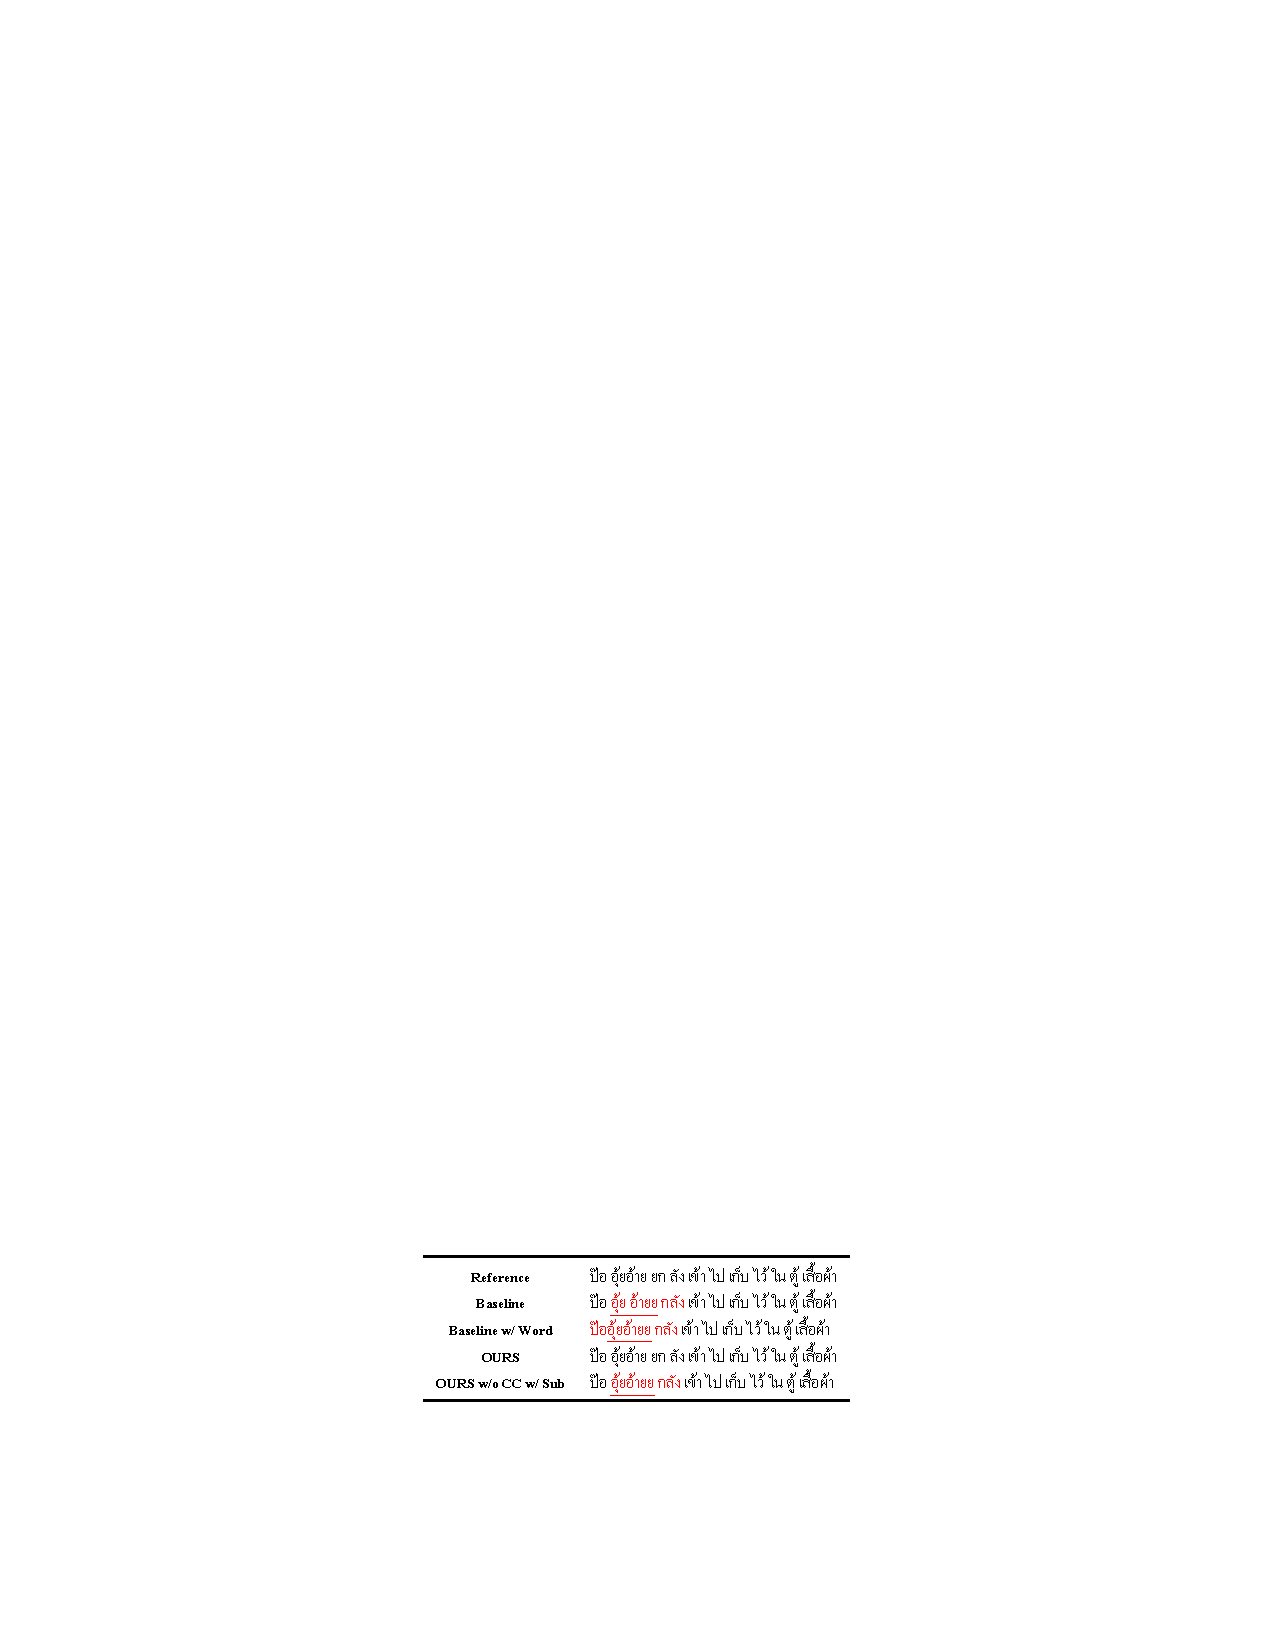
\includegraphics[width=0.6\textwidth]{figures/fig-case-study.pdf}
    \hspace{\textwidth}
    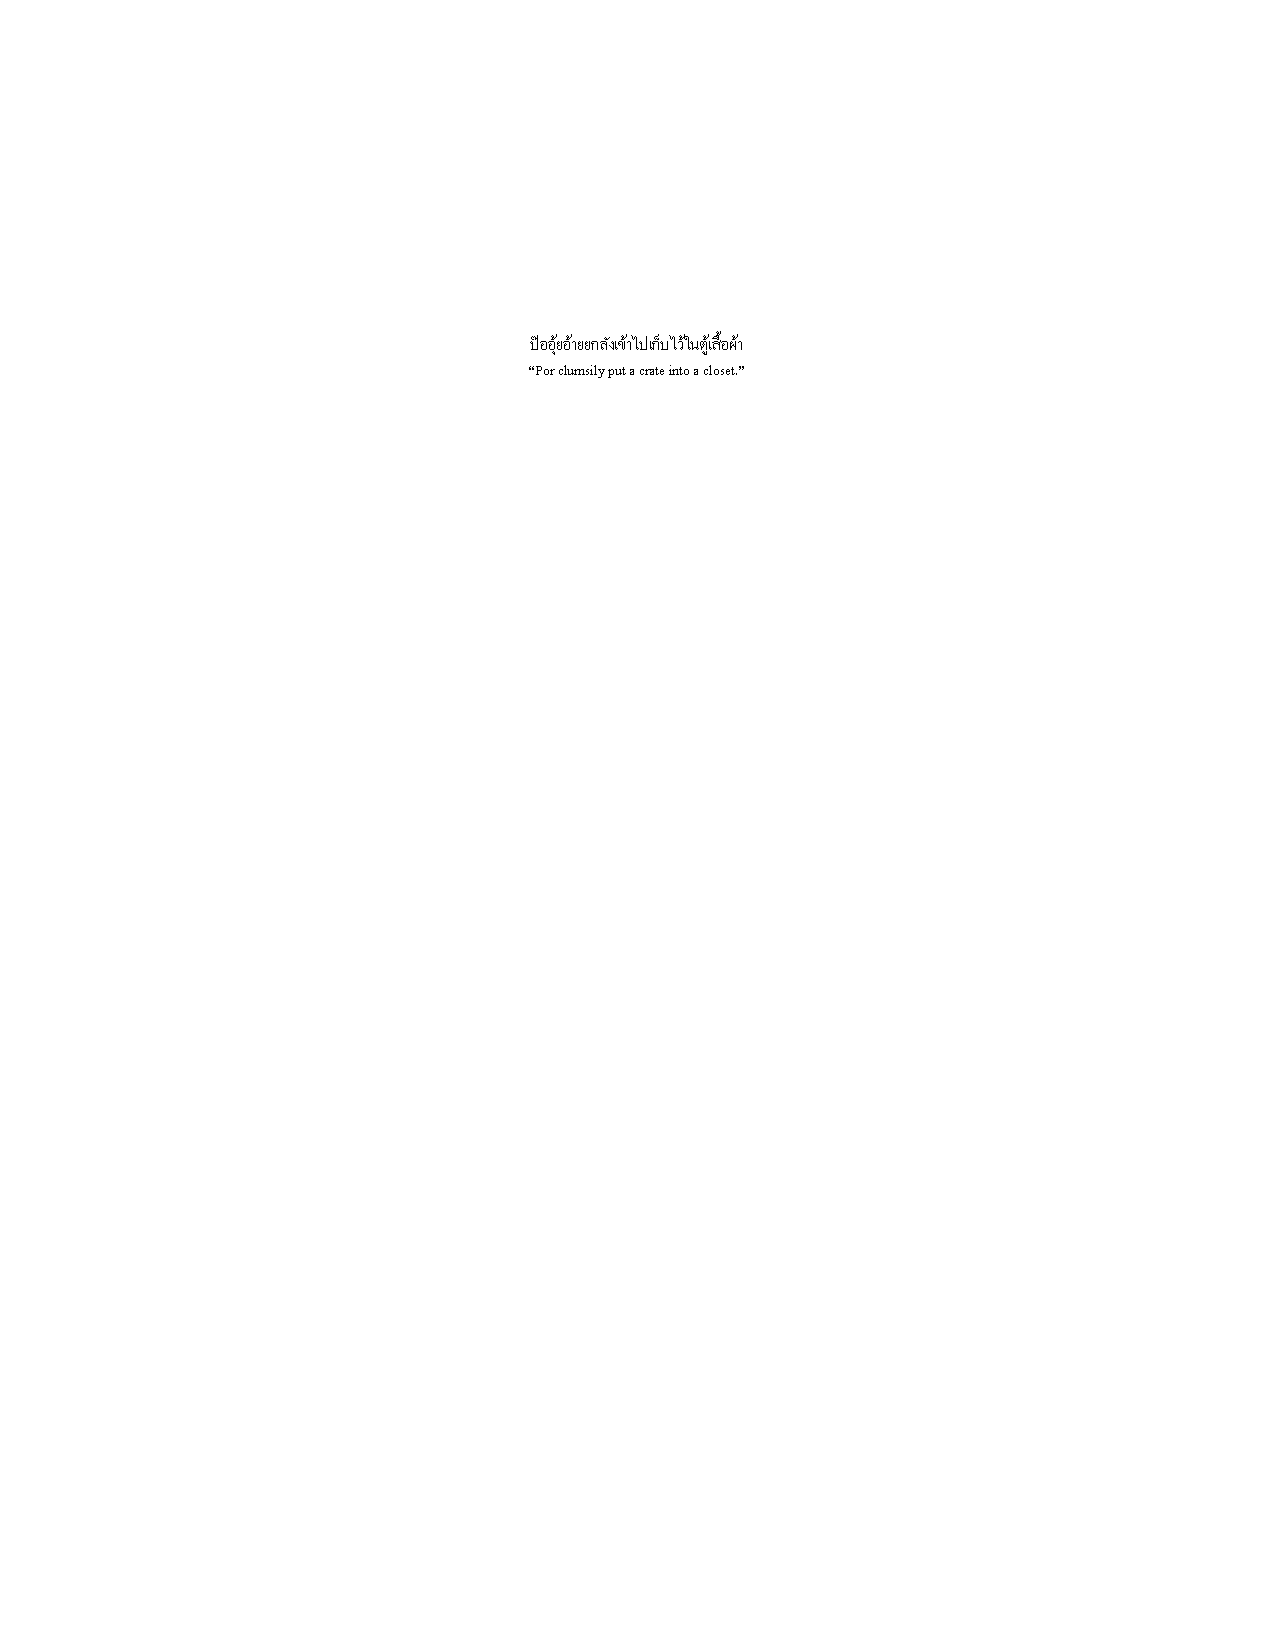
\includegraphics[width=0.35\textwidth]{figures/fig-case-study-tran.pdf}
    \caption{Examples of segmentation results among baseline models and our models. Ground-truth segmentation result is indicated as ``Reference'' and incorrect segmentation results are in \textcolor{red}{red}. \underline{underline} indicates segmentation results that violate Thai writing system.}
    \label{fig:case-study}
\end{figure}

\section{Conclusion and Future Work}
We proposed a character-based Thai word-segmentation model that uses multiple attentions on various types of linguistic knowledge, i.e., words, subwords, and CCs.
%
The best version of our model outperformed Thai state-of-the-art performance by using the word attention along with CC attention in the BiLSTM-CRF architecture.
%
The comparison between BiLSTM-based models with BERT-based models mostly showed that BiLSTM-based models surpassed BERT-based models, particularly by using our method.
%
However, our approach yet showed the improvement over the baseline model after integrating a pretrained BERT model into our proposed model.
%
Our further analysis also indicates that using CC can be more beneficial than using subword units in word-segmentation tasks.
%
As for future work, the multiple attentions can be merged into a single attention to reduce the model size as well as time complexity.
%
Furthermore, instead of using existing pre-trained models, building our own pre-trained models for fine-tuning the proposed model can also be considered.


%%%%%%%%%%%%%%%%%%%%%%%%%%%%%%%%%%%%%%%%
% Start Acknowledgment
\acknowledgment
This paper is an extended version of our preliminary paper \cite{chay-intr-etal-2021-character} presented in The $\text{13}^{\text{th}}$ Recent Advances in Natural Language Processing (RANLP 2021). 
%
In this paper, we add detailed explanations and the following new information to the original one: BERT and recent domain-dependent Thai word segmentation in introduction; pre-trained model in Thai word segmentation in related work; explanation of BERT layers in approach; four non-neural models for comparison; two new domain-dependent datasets with their statistics for comparing our model with recent domain-dependent models; hyperparameters for pre-trained model integration; experimental results for pre-trained model integration, comparison of our model and recent Thai domain-dependency works on two domain-dependent datasets; analysis for pre-trained model integration results and domain-dependent comparison; population standard deviation in neural models; statistical significance tests for the strong baseline models on main results and analysis. 
%

% Start bibliography
\bibliographystyle{jnlpbbl_1.5}
\bibliography{anthology,e_yourrefs}

% % Start biography
% \begin{biography}

% \bioauthor{Thodsaporn Chay-intr}{%
% He received his M.Eng. from Sirindhorn Institute of Technology, and is currently a doctoral student at Tokyo Institute of Technology. His current research interests are in Natural Language Processing, particularly text classification, computer linguistic, and text mining.
% }

% \bioauthor{Hidetaka Kamigaito}{%
% He received his Ph.D. from Tokyo Institute of Technology, and is currently an associate professor at Nara Institute of science and Technology. His current research interests are in Natural Language Processing with a specific focus on document-level text processing.
    % kamigaito.h@is.naist.jp
% }

% \bioauthor{Manabu Okumura}{%
% He received his Dr. Eng. from Tokyo Institute of Technology, and is currently a professor at Institute of Innovative Research. His current research interests include Natural Language Processing, especially text summarizing, computer assisted language learning, sentiment analysis, and text mining.
% }
% \end{biography}

%%%% \biodate   %%%% Following settings will be edited by editors.
\end{document}